\documentclass[pdftex,12pt,twoside]{book}
\RequirePackage[pdftex]{hyperref}
\hypersetup{colorlinks=true, %
  linkcolor=red,%  %% links within the doc e.g. ToC entries
  urlcolor=blue,%  %% links to the interwebs
  plainpages=false, %
  pdfpagelabels, %
  %hyperindex=true, %
  %backref=true, %
  %bookmarks=true, %
  pdftitle={Tech Fluency Labs for Math and Science Students, Version 0.1}, %
  pdfauthor={Len Brin, Joe Fields, Younhee Lee and Ray Mugno}, %
  pdfsubject={Computational tools for mathematics}, %
  %pdfpagelayout=SinglePage, %
  %pdfpagetransition=Dissolve, %
  pdfstartview=FitH, %
  %pdfstartpage=1, %
  %pdffitwindow=true
}
\pdfcompresslevel=9




\usepackage[Bjornstrup]{fncychap}


%All my customized LaTeX commands are in this file:

\usepackage[english]{babel} %language selection
\selectlanguage{english}
\usepackage{makeidx}
\usepackage{graphicx}
\usepackage{rotating}
\usepackage{amsmath,amssymb,amsthm,amscd,mathtools}
\usepackage{color}
\usepackage{enumitem}
\usepackage{ulem}
\usepackage[font=small,labelfont=bf]{caption}
\usepackage{subcaption}
\usepackage{tikz}
\tikzset{dot/.style={draw,shape=circle,fill=black,scale=.2}}
\usepackage{geometry}
\usepackage[pdftex]{hyperref}  %It has been claimed that hyperref should be loaded last...
\hypersetup{ %
  colorlinks=true, %
  linkcolor=red,%  %% links within the doc e.g. ToC entries
  urlcolor=blue,%  %% links to the interwebs
  plainpages=false, %
  pdftitle={Tech Fluency Labs for Math and Science Students, Version 0.1}, %
  pdfauthor={Len Brin, Joe Fields, Younhee Lee and Ray Mugno}, %
  pdfsubject={Computational tools for mathematics} %
}
\pdfcompresslevel=9

\makeatletter
\newcommand{\newreptheorem}[2]{\newtheorem*{rep@#1}{\rep@title}\newenvironment{rep#1}[1]{\def\rep@title{#2 \ref{##1}}\begin{rep@#1}}{\end{rep@#1}}}
\makeatother


\newcommand{\cents}{\textcent\kern 5pt}

\newcommand{\sageprompt}{ {\tt sage$>$} }
\newcommand{\tab}{\rule{20pt}{0pt}}
\newcommand{\blnk}{\rule{1.5pt}{0pt}\rule{.4pt}{1.2pt}\rule{9pt}{.4pt}\rule{.4pt}{1.2pt}\rule{1.5pt}{0pt}}
\newcommand{\suchthat}{\; \rule[-3pt]{.25pt}{13pt} \;}
\newcommand{\divides}{\!\mid\!}
\newcommand{\tdiv}{\; \mbox{div} \;}
\newcommand{\restrict}[2]{#1 \,\rule[-4pt]{.125pt}{14pt}_{\,#2}}
\newcommand{\lcm}[2]{\mbox{lcm} (#1, #2)}
\renewcommand{\gcd}[2]{\mbox{gcd} (#1, #2)}
\newcommand{\Naturals}{{\mathbb N}}
\newcommand{\Integers}{{\mathbb Z}}
\newcommand{\Znoneg}{{\mathbb Z}^{\mbox{\tiny noneg}}}
\newcommand{\Enoneg}{{\mathbb E}^{\mbox{\tiny noneg}}}
\newcommand{\Qnoneg}{{\mathbb Q}^{\mbox{\tiny noneg}}}
\newcommand{\Rnoneg}{{\mathbb R}^{\mbox{\tiny noneg}}}
\newcommand{\Rationals}{{\mathbb Q}}
\newcommand{\Reals}{{\mathbb R}}
\newcommand{\Complexes}{{\mathbb C}}
%\newcommand{\F2}{{\mathbb F}_{2}}
\newcommand{\relQ}{\mbox{\textsf Q}}
\newcommand{\relR}{\mbox{\textsf R}}
\newcommand{\nrelR}{\mbox{\raisebox{1pt}{$\not$}\rule{1pt}{0pt}{\textsf R}}}
\newcommand{\relS}{\mbox{\textsf S}}
\newcommand{\relA}{\mbox{\textsf A}}
\newcommand{\Dom}[1]{\mbox{Dom}(#1)}
\newcommand{\Cod}[1]{\mbox{Cod}(#1)}
\newcommand{\Rng}[1]{\mbox{Rng}(#1)}

\DeclareMathOperator\caret{\raisebox{1ex}{$\scriptstyle\wedge$}}

\newtheorem*{defi}{Definition}
\newtheorem*{exer}{Exercise}
\newtheorem{thm}{Theorem}[section]
\newtheorem*{thm*}{Theorem}
\newtheorem{lem}[thm]{Lemma}
\newtheorem{cor}{Corollary}
\newtheorem{conj}{Conjecture}

\renewenvironment{proof}%
{\begin{quote} \emph{Proof:} }%
{\rule{0pt}{0pt} \newline \rule{0pt}{15pt} \hfill Q.E.D. \end{quote}}

\newenvironment{worksheet}[3]{%
\begin{tabular*}{6in}{l @{\extracolsep{\fill}} r} \hline %
\begin{tabular}[c]{l} %
 {\huge Lab: #1} \\%    %% #1 is a sequence number (should be done automagically, but...  reasons)
{\rule{0pt}{22pt}\LARGE #2} \\%        %% #2 is the title of the activity
\end{tabular} &  \begin{tabular}[c]{r} %
\rule{0pt}{1.05in}\includegraphics[height=1in]{#3} \\%  %% #3 is a thumbnail image for the activity
\end{tabular}  \\ \hline%
\end{tabular*}%
\par \rule{0pt}{6pt} \par \noindent }{ \vfill \centering 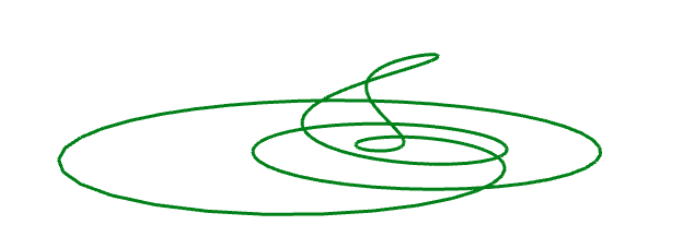
\includegraphics[height=1in, width=5in]{lab_end.png} \clearpage}

\newenvironment{codeblock}{ \par \rule{0pt}{12pt} \par \hfill \begin{minipage}{0.9\textwidth} }{ \end{minipage} \par \rule{0pt}{12pt} \par }

\renewcommand{\baselinestretch}{1.2}
\renewcommand{\arraystretch}{.83}

\graphicspath{{../figures}{figures}}



%Things that effect the size and placement of text on the page

\renewcommand{\baselinestretch}{1.2}
\renewcommand{\arraystretch}{.83}

%\addtolength{\topmargin}{-.5in}
%\addtolength{\textheight}{1.25in}
%\addtolength{\textwidth}{.25in}
%\addtolength{\oddsidemargin}{.25in}
%\addtolength{\evensidemargin}{-.25in}

%\usepackage[bottom=1in, right=1in, left=1in, top=1in]{geometry}
\usepackage[  
    letterpaper,
    bindingoffset=0.875in,
    textwidth=6.25in,
    top=1in,
    bottom=1in,
    showframe
]{geometry}

\makeindex

\graphicspath{{figures/}}

\begin{document}

\frontmatter

\title{Technological Fluency Labs \\ for Math and Science Students, \\ Version 0.1}
\author{Len Brin, Joe Fields, Younhee Lee and Ray Mugno}
\date{\em \small Southern Connecticut State University}

\maketitle

\clearpage

\rule{0pt}{0pt}

\vfill

\begin{quote}
    Copyright \copyright{}  2023  Len Brin, Joe Fields, Younhee Lee and Ray Mugno.
    Permission is granted to copy, distribute and/or modify this document
    under the terms of the GNU Free Documentation License, Version 1.3
    or any later version published by the Free Software Foundation;
    with no Invariant Sections, no Front-Cover Texts, and no Back-Cover Texts.
\end{quote}

\vfill


\clearpage

%\rule{0pt}{0pt}

%\vfill

%\begin{quote}
%{\Large \bf Acknowledgments} 
%\end{quote}

%\vfill


%\clearpage

\tableofcontents

%\listoffigures

%\listoftables

\chapter*{Preface}
\chaptermark{Preface}

The goal of this book is to help you learn about a variety of 
computational tools that will be useful in your career as a mathematician
or scientist.


\mainmatter

 
\chapter{Introduction}

This book aims to introduce the reader to several computational tools that are useful for people entering careers in Mathematics and the Sciences.  We have chosen to emphasize systems that are open-source but we generally indicate other options in the introduction to each chapter.

The book is divided into 8 main chapters.

\begin{itemize}

\item This Introduction.

\item Writing with embedded mathematical content.

\item Computational Algebra.

\item The creation and inclusion of Graphics in technical documents.

\item Interactive Geometry.

\item A chapter on the use of Spreadsheets.

\item Statistics

\item Miscellaneous

\end{itemize}

In each of those chapters there will be technological as well as mathematical learning goals.  The point of this book is to collect laboratories/activities that will allow one to reach these goals through an active learning strategy: doing stuff, not being told about it! 

An important aspect of developing a facility with tech is that you get better at it the more you do it.  Many people advocate that ``learning how to learn'' is one of the biggest benefits of a college education.  So we hope that part of the takeaway from doing these labs is that it will be easier for you to figure out other tools that you'll encounter in the future.  For example, a great many computer applications allow you to access their functionalities via a menu system.  Many of those menu entries have a keyboard shortcut associated with them.  Once you see the increased productivity you get from using such shortcuts, you start to look for them in other applications.  And, there are fairly consistent conventions about how those shortcuts are selected so knowledge you gain in one app often transfers over directly to others!

In the early days of computing, someone introduced the initialism RTFM which doesn't really stand for ``Read that fine manual.''  That's one piece of advice that you should certainly take away from the TFLabs experience -- learn how to access and read the help facility!  A couple of other suggestions for getting up to speed quickly in a new computing environment:

\begin{itemize}
	\item Often, the help for a particular command will include examples.  Scrolling past that wall of confusing text until you get to the relevant examples isn't a terrible strategy.
	\item See if there are so-called ``tool-tips'' -- hovering your mouse over a button often causes a pop-up that displays a hint about what the button does.
	\item Look for the aforementioned keyboard shortcuts.  A lot of programs use Ctrl-Z as a shortcut for ``undo'' (this can be super useful!  Unless the command is Ctrl-U in your particular application.)
	\item Learn to read error messages.  These messages are generated programattically when something goes wrong - this usually makes them a bit cryptic.  If you're able to crack the code, you'll probably at least get a hint as to what caused the problem.
	\item Use your favorite search engine to see if there is relevant help already out there.  ``Hey Siri, how do I get an ampersand in LaTeX?''  (I really don't know if that will work, but putting that question in my browser's search bar sure does!)
	\item Doing the previous ``googling'' will often lead you to online help fora like Quora, Reddit and Stack Overflow.  Reading threads in a forum can be really helpful.  Posting questions in a forum is hit-or-miss -- sometimes you'll get a quick useful answer, other times the result is not what one would want\textellipsis  
\end{itemize}

Let's get started!


 
\chapter{Writing}

\section{HTML}
\label{sec:html}

Have you ever seen a web URL like 
\begin{center}
\href{https://www.agnesscott.edu/lriddle/women/love.htm}{\tt https://www.agnesscott.edu/lriddle/women/love.htm}
\end{center}

\noindent and wondered what the \texttt{https} or the \texttt{htm}
meant? In both \texttt{https} and \texttt{htm}, the \texttt{ht} is
short for hypertext. The \texttt{tp} in \texttt{https} is short for
transfer protocol and the \texttt{s} is for secure. The \texttt{m}
in \texttt{htm} is for markup. All webpages, when it comes down to
it, are made of HTML (hypertext markup language) code. The HTML tells
the browser what should be displayed and, in general terms, the desired
layout. The browser takes care of the fine details depending on the
type of device, size of the screen, or personal preferences set by
the user.

Markup in HTML is like a note to the browser telling the browser how
to display the following content. The markup won't be displayed, but
it will modify how the content will be displayed. Take this screenshot
from \texttt{\href{https://www.southernct.edu/}{https://www.southernct.edu/}}
for instance.
\begin{center}

\includegraphics[width=4in]{write/SCSUscreenshot}
\par\end{center}

\noindent Simplified just a bit, the HTML code that produces the ``Back
to Campus'' announcement above looks like this:
\begin{verbatim}
<img src="/sites/default/files/back-to-campus-banner.jpg" /><p style
="font-size: 18px;">As the university prepares for the start of the
fall 2021 semester, we remain #SouthernStrong, with <a href="https://
inside.southernct.edu/reopening#services">all of the following academic
offerings and campus services</a> in place for our students in a safe,
engaging campus environment. Our goal is to get you off to a great
start, whether you're returning to campus or joining our community for
the first time!</p>
\end{verbatim}

\noindent It is just simple text! No bells, no whistles. Parts enclosed by \texttt{<}
and \texttt{>} are the markup. These parts will not be displayed themselves
but rather describe how something is to be displayed and leaves the
rest up to the browser. For example,

\begin{center}
\verb+<img src="/sites/default/files/back-to-campus-banner.jpg"/>}+
\par\end{center}

\noindent tells the browswer to insert an image ({\tt img}) and
tells the browser where to get the image ({\tt src}). This part
of the code creates

\begin{center}

\includegraphics[width=4in]{write/back-to-campus-banner}
\par\end{center}
  
\noindent The rest of the code creates the paragraph underneath this
image. It starts with \verb+<p style="font-size: 18px;" >+ --- which
tells the browser to start a paragraph ({\tt p}) using an 18 pixel
font---and ends with \verb+</p>+, which tells the browser this
is the end of the paragraph. In the middle of the paragraph is what
makes webpages webpages---a hyperlink. The text between 
\verb+<a href="https://inside.southernct.edu/reopening\#services" >+
and \verb+</a>+ is marked up as a link, it's displayed in blue so the reader can see that
these words are where they can click. Clicking them will bring up a new webpage in
the browser.
\clearpage

\begin{worksheet}{1}{Working with markup}{figures/html.pdf}
To see markup in action, point your browser to 

\centerline{ \texttt{\href{https://htmledit.squarefree.com/}{https://htmledit.squarefree.com/}}, }

\noindent where you can write some hypertext markup and see how it looks on
your browser. The blue box at the top holds the markup, and it can
be edited by you! The box below shows how the browser renders the
markup. Do the following exercises on the \texttt{squarefree} webpage
and answer the questions.
\begin{enumerate}
\item Insert \texttt{<em>} before the word magically and insert \texttt{</em>}
after the word magically. What did this accomplish? Note: \texttt{em}
is short for \textit{em}phasis!
\item Copy and paste the following code into the webpage.

\begin{verbatim}
<p>A list of some common HTML markup
<ol>
 <li><tt>p</tt> is short for <b>p</b>aragraph</li>
 <li><tt>a</tt> is short for <b>a</b>nchor (which can
indicate a link or a place to link to)</li>
 <li><tt>ol</tt> is short for <b>o</b>rdered <b>l</b>ist</li>
 <li><tt>li</tt> is short for <b>l</b>ist <b>i</b>tem</li>
</ol>

Notice that markup can be nested -- the b and /b tags above are
inside the li and /li tags, which are between the ol and /ol
tags.</p>
\end{verbatim}


\item What happens to text between the \texttt{<b>} and \texttt{</b>} tags?
\item What happens to text between the \texttt{<tt>} and \texttt{</tt>}
tags?


\item Now change the \texttt{<ol>} and \texttt{</ol>} tags to \texttt{<ul>}
and \texttt{</ul>} tags. What happens to the displayed page (in the
white box)? Note: \texttt{ul} is short for \textbf{u}nordered \textbf{l}ist.

Make a new ordered list and use it to store your answers to the lab questions \#1, \#2, etc.

\item Notice how the b and /b tags in the last sentence of the copy/pasted code above are missing the usual angle brackets.  What happens if you put them in?
\item This is a problem in all markup languages -- some characters have special meaning.  In HTML there are so-called {\em escape characters} to work around this issue.  Google the phrase ``html escape characters'' and see if you can re-write the last sentence so that things {\bf look like} a tag, but don't {\bf act like} a tag!
\item Look up how to use the \texttt{<a href="...">...</a>} and \texttt{<img src="..."></img>} tags to make a link to another website and embed an image in your page.
\item Try writing some text and put a single \texttt{<br>} tag somewhere. What happens? Why doesn't it need a ``closing'' tag?
\item Similarly, what does the \texttt{<hr>} tag do?
\item There are lots of different computer programs (``browsers'') that need to translate the html source code of the webpages you visit into the beautiful layouts you see on your screen. How many different browsers can you think of?
\item Who is in charge of deciding what those browsers need to recognize as official html code? (Hint: search the internet for ``W3C.'') Who is in charge of that organization, and where do its profits go?
\end{enumerate}
\end{worksheet}

\section{LaTeX}
\label{sec:latex}

Donald Knuth is an amazing Zen master of Computer Science and Mathematics.  He created a program called \TeX (pronounced like ``tech'') for typesetting -- especially typesetting with mathematical content.  Knuth wrote \TeX mainly as an example of a style of coding that he called ``literate programming.''  Essentially this means that the programmer creates the documentation for their work at the same time they write the actual code.  Whether it's because of it being written in the ``literate programming'' style or simply because of Knuth's amazingness, \TeX\  is renowned as one of the most bug-free systems in existance. 

\TeX\ , and a follow-on program known as \LaTeX\ , which builds on \TeX\  and extends it, have become the standard(s) for communicating mathematics.  We'll be talking only about \LaTeX\ from here onward.  \LaTeX\ is much like HTML -- it is a sort of markup language that gets processed and turned into a document suitable for visual display.  The appearance of \LaTeX source code is very different from that of HTML source code, but in many ways they are incredibly similar!  There are two marked distinctions:  HTML is meant to describe how to lay out a page so that the content is clear, and do so on many different displays -- the web-browser is empowered to alter things to aid in that clarity. On the other hand, \LaTeX is much more focussed on layout -- the first thing one does in a \LaTeX document is to specify the page size.  The author of a \LaTeX document can closely control where things will end up on that page\footnote{There is a strong argument against doing so -- the author should really concentrate on content, and let the software control the individual pixels on the page.}.
The other big difference between these systems is how well they handle mathematical content.  \LaTeX is very, very good at rendering mathematics and mathish notation from other fields like Chemistry.  HTML stinks at that, which is completely weird since the original HTML standard was created by a physicist at CERN, and physicists tend to use a lot of math\textellipsis

In a nutshell, HTML (the markup language of webpages) is used to
control how a webpage appears. \LaTeX\  plays the same role for printed
documents like books, reports, letters, or labs (like this one!).
\LaTeX\  is a markup language that excels at creating technical documents,
especially those that include mathematical formulas. You might want
to read \href{https://medium.com/swlh/the-students-guide-to-latex-markup-what-it-is-and-why-you-want-it-651e723ce0c8}{this blog}
all about why you want to learn \LaTeX.

Like HTML, \LaTeX\  uses tags to mark how text should look, to insert
graphics, to create lists, and so on. Markup in \LaTeX\  begins with
a \textbackslash{} (a backslash) as in {\tt \textbackslash pi},
which would be used to render our friend, $\pi$. Every \LaTeX\ 
document begins with the {\tt \textbackslash documentclass} tag,
which specifies what type of document is to be created (book, article,
report, etc.).  This is similar to HTML documents, which all begin with the \verb+<html>+
tag and end with the \verb+</html>+ tag. After the documentclass tag a \LaTeX\  document must include the
tags {\tt \textbackslash begin\{document\}} and {\tt \textbackslash end\{document\}}.\footnote{This is similar to HTML documents, in which the beginning of the content
is marked by {\tt <body>} and the end by {\tt </body>}.} As you can probably guess, these tags mark the beginning and end
of the content of the document. One of the simplest \LaTeX\  documents
possible is this one:

\begin{codeblock}
\begin{verbatim}
\documentclass{article}
\begin{document}

Hello World!

\end{document}
\end{verbatim}
\end{codeblock}

Just like HTML code, it isn't pretty! However, it tells the \LaTeX\ 
renderer what to do. This code will create an ``article'' with the
sentence ``Hello World!'' in it. 

Let's give it a try!

The next lab will lead you through the process of creating \LaTeX documents on a web-based service known as {\em Overleaf}.

\clearpage
\begin{worksheet}{2}{Getting started with \LaTeX}{figures/latex.pdf}
\begin{enumerate}
	\item Go to \href{https://www.overleaf.com/register}{\tt https://www.overleaf.com/register}
	\item Register for a free account (probably best to use your university email.)  You'll have to create a password at this point - make a note of it.\footnote{Overleaf isn't exactly a ``high stakes'' setting, your password needn't be super complicated -- just don't re-use a password that protects a more critical account!}
	\item It's probably best to skip their ``Try the premium version for free'' offer.
    \item Click the ``Create First Project'' button -- choose a blank project and name it ``hello.''
    \item You'll see two main panels (there's also some junk above and to the left, but ignore all that for now.)  The left-hand panel contains the \LaTeX\ source code for your project and the right-hand panel gives a preview of the resulting document.
    \item The ``blank project'' isn't completely blank.  The source code panel will be pre-populated with:
\medskip

\begin{codeblock}
\begin{verbatim}
 \documentclass{article}
 \usepackage{graphicx} % Required for inserting images

 \title{hello}
 \author{myemail}
 \date{August 2023}

 \begin{document}

 \maketitle

 \section{Introduction}

 \end{document}
\end{verbatim}
\end{codeblock}

\clearpage

You should see your document on the right side. It has a title section (which is 
what the \verb+\maketitle+ command created) and a section heading (this is what the \verb+\section{Introduction}+ command did). Scroll down to the bottom of the page and you
will see the number 1, the page number. Pages of articles are normally
numbered, so \LaTeX\  puts that in for you!  The area
between the \verb+\documentclass{article}+ and
the \verb+\begin{document}+ tags is known
as the \textbf{preamble} of the \LaTeX\  document. 
You should see that the preamble contains some commands that effect how the title looks.  
The default stuff that Overleaf stuck in there probably isn't quite what you want.

Let's fix that!


\item Make whatever changes you deem appropriate to the title, author and date commands. (BTW, ``date'' doesn't necessarily have to literally be the date.)  To see what the effect of your changes is, you'll need to press the ``Recompile'' button.

\item Put some words, introducing yourself after the \verb+\section{Introduction}+ command, and recompile. (There is an old and slightly unfunny tradition that the first program you write when learning a new programming language is called ``hello world!''  Please make your introduction something other than that.)

\end{enumerate}

At this point the source code might look something like:
\bigskip

\begin{codeblock}
\begin{verbatim}
\documentclass{article}
\usepackage{graphicx} % Required for inserting images

\title{My first LaTeX document}
\author{Ima Dumi}
\date{just checking that I can put whatever I want in the date}

\begin{document}

\maketitle

\section{Introduction}

Something other than that.

\end{document}
\end{verbatim}
\end{codeblock}

\clearpage

Which should render like so:


\begin{center}
\fbox{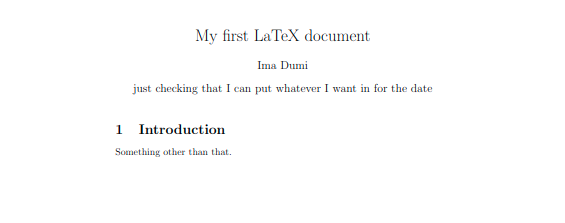
\includegraphics[width=6in]{HelloWorldScreenshot.png}}
\end{center}


\subsection*{Adding a list}

Now add a list of your three favorite classes of all time---of course
math class is first on your list, so that one has been put in for
you. You'll have to supply the next two...

\begin{enumerate}

\item Copy and paste the following markup into your document 
after your greeting, but before \verb+\end{document}+.
\bigskip

\begin{codeblock}
\begin{verbatim}
\par
My three favorite classes of all time are

\begin{enumerate}
  \item Math
\end{enumerate}
\end{verbatim}
\end{codeblock}
\bigskip

Notice that the \verb+\par+ tag does not have a begin
or end. It only marks where a new paragraph should start. Same with
the \verb+\item+ tag. It only marks where a new item
in the list should start.
\item Add two items to the enumeration (and you can change the first item
if by some strange chance math is not your all time favorite class).
\item There are several list-making environments in \LaTeX.  Try some googling (Maybe ``list making latex environments'') 
and you should discover the other list-making environments.
\item Make version of your list of favorite classes that are (1) bulleted rather than numbered, (2) name the class and also give a comment about \sout{why math is so awesome} why you like it.

\end{enumerate}

\subsection*{Adding an equation}

Equations in \LaTeX\ come in two varieties---inline and display.
An inline equation is any mathematical expression that appears in
the middle of a sentence (like the $\pi$ right here and earlier in
this document). A display equation is any mathematical expression
that should appear centered on its own line (because it's super important
or just because it's too big to put in the middle of a sentence).

To put an equation in the middle of a sentence, enclose the math between
two dollar signs (\$). To add a display equation, enclose the math
between double dollar signs (\$\$). Try it!

\begin{enumerate}
\item Copy and paste the following markup into your document.
\bigskip

\begin{codeblock}
\begin{verbatim}
My favorite mathematical constant is $\pi$, but I like $e$ too.
Did you know that $$e^{i\pi}=-1?$$ Weird...
\end{verbatim}
\end{codeblock}
\bigskip

\item Notice that exponents are typeset using the same notation as used
on a calculator! Can you add markup to your document that will produce
the following?

\begin{quote}
The Pythagorean Theorem states that if a triangle has legs of lengths
$a$ and $b$ and hypotenuse of length $c$, then
\[
a^{2}+b^{2}=c^{2}.
\]
\end{quote}

\end{enumerate}

\end{worksheet}



\section{MathJax}
\label{sec:mathjax}

\section{More Markup (Blogs and Wikis)}
\label{sec:markup}


 
\chapter{Spreadsheets}


\section{Libr\'{e} Office Calc}
\label{sec:calc}

\subsection{Introduction}


Spreadsheets were one of the original ``killer apps'' when personal computers were first introduced.  Spreadsheets allow you to deal with tables of numbers and other data.  The standard convention is that the rows of a spreadsheet are indexed by numbers and the columns are indexed with letters.  If you need to go past 26 columns, use AA, AB, AC, {\em et cetera} for the next several columns.  It would be pretty unusual to need to have more than 702 columns but if you needed to, guess what comes after ZZ.

We're going to be using the free/open-source Libr\'{e} Office spreadsheet in the upcoming labs.  There are other choices (Excel on Windows and Numbers on Apple computers) but all of them work in a similar way and Libr\'{e} Office is free.  Spreadsheet files created by 
Libr\'{e} Office have a .ods suffix.  

To load Libr\'{e} Office on your personal machine, visit \url{https://www.libreoffice.org/download/download-libreoffice/}

\clearpage
\begin{worksheet}{11}{Intro to Spreadsheets}{LibreCalc.png}
If you haven't done so already, visit \url{https://www.libreoffice.org/download/download-libreoffice/} and download the Libr\'{e} Office suite.

Suppose a businessman was in the completely legitimate business of making loans to people who are regarded as poor credit risks by conventional banks.  Of course, he'd want to keep track of the loan amounts and the recipients.  A spreadsheet is the perfect tool!

Here's a screen shot of how the data might be recorded:

\centerline{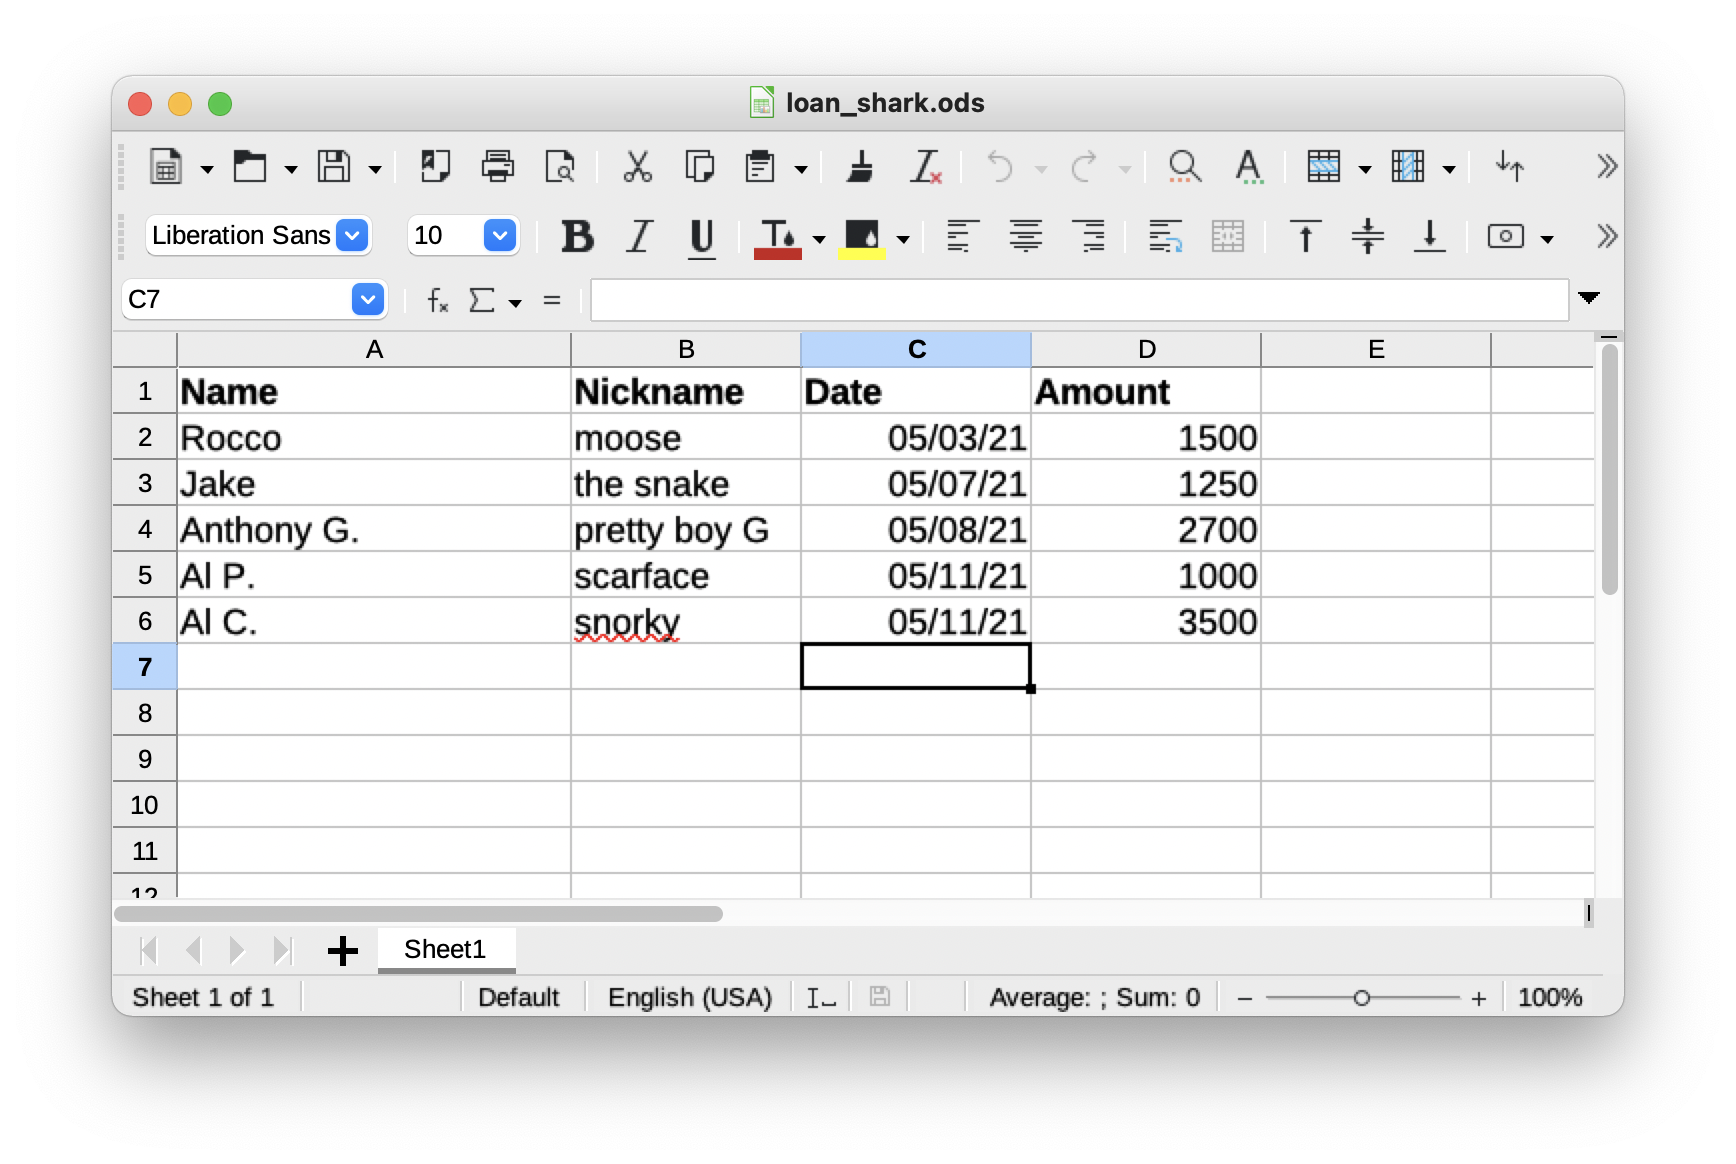
\includegraphics[scale=.5]{loans.png}}

We're using the free/open-source Libr\'{e} Office spreadsheet in the above.  There are other choices (Excel on Windows and Numbers on Apple computers) but all of them work in a similar way and Libr\'{e} Office is free.  Spreadsheet files created by Libr\'{e} Office have a .ods suffix.  

The stuff that you enter into a cell in a spreadsheet fall into two main categories: a cell can contain data, or a cell can contain a calculated value.  To make a ``calculation''-type cell you have to put an equals sign up front.  When you're doing a calculation you can use the values that are in other cells by referring to them by column (letter) followed by row (number).  For example the \$3500 that Snorky borrowed is in cell D6.

Some calculated cells are pretty simple, like the sum, difference or product of the values in other cells.
Other calculated cells can be pretty complex -- there are a lot of built-in functions that can be used to do these more difficult computations.  Once you know your way around, you'll probably just type the name of the function you need.  Until then there is the so-called ``function wizard.''  Try looking for a function that will give you random numbers.

\centerline{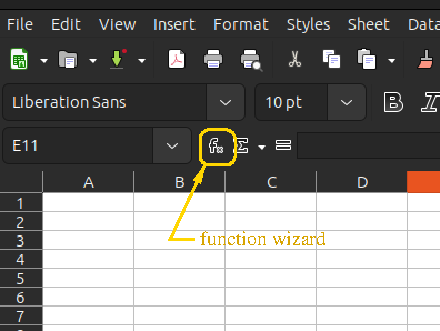
\includegraphics[scale=.5]{func_wiz.png}}

\subsubsection{tasks}

\begin{enumerate}

\item Open the loan shark spreadsheet (the file is available on the book website) and make some additions -- columns for monthly interest rate, due date and the current amount due.  You should verify that subtracting the values in two cells that are formatted as dates does the right thing.  Since you'll want time to be measured in months, what conversion needs to be applied?

\item Create a spreadsheet for keeping track of student grades in a math class. Use your favorite actors, sports stars, musicians (or whatever) as students, and just generate random numbers to put in as their grades. Make the homework grades (let's say 5 different scores) be on a scale from 0 to 10.  Make the quiz grades (also 5 of them) be on a scale from 0 to 20. Finally, make up two exam scores on a 0 to 100 scale.
Create subtotals for homework, quizzes and exams, also a grand total with homework weighted $20\%$, quizzes weighted
$30\%$ and exams weighted $50\%$.  

Many teachers have policies where the lowest grade in some category is dropped.  Figure out how to drop the lowest quiz score.

\end{enumerate}


\end{worksheet}
\clearpage


\subsection{Absolute and relative cell references}

\subsubsection{tech}

If you're going to be using the same calculation in a bunch of different places, you can just copy and paste the contents of one cell into another.  Get used to using the keyboard shortcuts Ctrl-C and Ctrl-V for copy and paste.  

When you copy and paste a formula, the spreadsheet intelligently changes the cell references in the formula.  The pasted formula refers to cells that are in the same positions {\em relative} to the spot we're pasting into.  

For example, if you type {\tt =B3 + C2}  into cell {\tt C3} you're telling the system to add the number just above and the number just to the left.  If you copy and paste that formula into cell {\tt K7} you'll find that the formula has become {\tt =J7+K6} because those cells are in the same relative positions.

This intelligent pasting {\em usually} does the right thing, but occasionally we really just want the thing to stay put!  If you want a cell reference to {\em not} change when you're cutting and pasting (this is known as an absolute reference) put dollars (\$) in front of both the letter and the number.  Very occasionally we want a sort of hybrid behavior -- we can put the dollar on one but not the other.  For instance, if in a formula we refer to a cell using \$A3  (with the dollar on the A but not in front of the 3) when we copy and paste the A will stay an A, but the 3 will change appropriately.  Some people call this making either the row or the column ``sticky.''  

\subsubsection{math}

In today's activity we'll be looking at two mathematical concepts: binomial coefficients and difference tables.

Binomial coefficients are sometimes called {\em choice counters}.  For example, given a set of 5 options how many ways can we select 3 of them?  This would be the binomial coefficient $\binom{5}{3}$ which is equal to 10.  To pronounce that symbol in English use the word ``choose,''  so the symbol above is read as ``five choose three.''  That notation for binomial coefficients can be a little confusing since many people assume the fraction bar just got left off!  So be careful, $\binom{5}{3} \; = \; 10$, but $\left( \frac{5}{3} \right) \; = \; 1.666\ldots$  so (obviously) these are different -- don't imagine fraction bars where they don't actually appear!

There is another notation for the same quantities using a capital letter $C$.  To indicate ``five choose three'' in this notation write $_5C_3$.

So why are these choice counters called ``binomial coefficients''?   It turns out these numbers also appear when taking powers of a {\em binomial} -- a polynomial with just two terms.  Try computing $(x+1)^0$, $(x+1)^1$, $(x+1)^2$ and $(x+1)^3$.  Really, only the last of those is at all difficult!  Anything to the $0$ power is just $1$, anything to the $1$ power is itself, and the $2$nd power just requires the FOIL rule!

Blaise Pascal -- a French mathematician who was one of the founders of the field of probability -- was probably the first to notice the pattern when you write these things next to one another.


\begin{tabular}{c}
	$1$ \\
	$x+1$ \\
	$x^2+2x+1$ \\
	$x^3 + 3x^2 + 3x+1$\\
\end{tabular}

The pattern becomes easier to deduce if you remove all the powers of $x$ (and the plus signs) and just concentrate on the coefficients.

\begin{tabular}{c}
	$1$ \\
	$1 \quad 1$ \\
	$1 \quad 2 \quad 1$ \\
	$1 \quad 3 \quad 3 \quad 1$\\
\end{tabular}

 Numbers on the outside of each row are always 1.  Numbers in the middle of a row are just the sum of the two things above them.
 
 The arrangement of binomial coefficients into this triangular array is called Pascal's triangle.  Here's the first 5 rows:
 
 \begin{tabular}{c}
 	$1$ \\
 	$1 \quad 1$ \\
 	$1 \quad 2 \quad 1$ \\
 	$1 \quad 3 \quad 3 \quad 1$\\
 	$1 \quad 4 \quad 6 \quad 4 \quad 1$\\
 	$1 \quad 5 \quad 10 \quad 10 \quad 5 \quad 1$\\
 \end{tabular}
 
 Difference tables come from a very common form of analyzing a sequence.
 
 Suppose we asked, ``What comes next?'' in the following sequence.
 
 \[ 4, \quad 7, \quad 10, \quad 13, \ldots \]
 
 You probably notice rather quickly that successive terms in the sequence differ by the same number.  A difference table is just a formalized way of making the same observation -- except that if the differences don't seem to have an obvious pattern we might continue on taking the differences of the differences!
 
 Here's an example.  Suppose you're given the following sequence of numbers.
 
 \[ 2 \quad 5 \quad 12 \quad 23 \quad 38 \quad \ldots \]
 
 A difference table looks like so:
 
 \begin{tabular}{ccccccccc}
 	2 &  & 5 & & 12 & & 23 & & 38 \\
 	   & 3 & & 7 & & 11 & & 15 
 \end{tabular}

SInce the differences don't exhibit an obvious pattern we continue on, obtaining

\begin{tabular}{ccccccccc}
	2 &  & 5 & & 12 & & 23 & & 38 \\
	& 3 & & 7 & & 11 & & 15 & \\
	& & 4 &  & 4  &  & 4 & & \\ 
\end{tabular}

It looks as though the bottom row -- which is known as the {\em second differences} is always 4.  Can you use that to predict what the next term in the sequence will be?

\subsubsection{tasks}

Write out the expanded form of $(x+1)^5$.

Create a table of the binomial coefficients $\binom{n}{k} = \frac{n!}{k!(n-k)!}$.

Revisit the grade spreadsheet from the previous section and insert a new row at the top.  Put the "weights" for homework, 
quizzes and exams into cells in this row.  (As the teacher you might want to experiment with different 
weighting schemes.) Are the final grades changed by much if we change the weights to 10, 
20 and 70 percent respectively?


Use a spreadsheet to do a finite differences analysis of the following sequence:

	  \[ 1 \quad 3 \quad 7 \quad 13 \quad 21 \ldots \]

Find the "back diagonals" for the sequences of squares, cubes, 4th powers etc.
(We care about back diagonals because you can use them to generate the entire sequence! (under the assumption that the bottom-most number is a constant) (sorry about all the parentheses)).

Maybe:
Given that the back diagonal for $x^n$ contains $s(n,k)*k!$ in the $k$th row, and the recursion for
the Stirling numbers.  Use a spreadsheet to create a table of the Stirling numbers.

\subsection{Builtin functions}

Tasks:

Returning to our gradebook example$\ldots$

Use the MIN function to "drop the lowest quiz."

Use functions to assign letter grades with $+$ and $-$ modifiers.

 
\chapter{Geometry with GeoGebra}


\section{Introduction to GeoGebra}
\label{sec:geogebra}

GeoGebra is an open source tool that lets you do geometric constructions and also work with algebraic expressions (Hence the Geo and the Gebra in the name).

GeoGebra is available as a an app for your phone, or your computer, or you can just access it via a webpage: \url{https://www.geogebra.org/}.

For doing the labs in this chapter it will be easiest to just use the web interface.  If you want to be able to save your work and/or share your work with others (trust me, this is something you'll want to do) you need to sign in.  You can use an existing sign-on, like Google or Facebook, or you can create a free GeoGebra account.  

Once you are signed in, go to the ``Home'' area and click the ``Start Calculator'' button.

At the top of the page, in the center, there is a selection box that lets you switch between 5 different versions of the GeoGebra calculator.  When you first start the calculator it will be in ``Graphing'' mode.  At the left side of the header area you'll see a ``hamburger'' that lets you access the top-level menu for the app.

\clearpage
\begin{worksheet}{14}{Intro to GeoGebra}{GeoGebra.png}
\begin{enumerate}

\item Start GeoGebra, sign in, and change the mode from ``Graphing'' to ``Geometry''

The interface will now have two large panes.  On the right is the drawing area.  On the left is where you can select from a bunch of different tools.

One source of annoyance is that the system does whatever action is dictated by the tool that is currently active.  So, for example, if you've selected the ``Point'' tool and you then try to move the view, you'll create a point that you hadn't really intended\ldots

One day you'll get used to this, but in the meantime there's an ``undo'' button\ldots

They've recently added a shortcut to get back to the ``Move'' cursor (since that's the most frequent switch we'll want to make, this is very handy)
\vfill

\item When you first enter the ``Geometry'' mode the tool panel will have a very limited number of options.  Expand them by clicking ``More.''  That gives you quite a few more possible tools to use, but at the bottom of the panel you'll find another ``More'' button.  After you click that one, every option will be displayed.  Look through the list of tools and figure out how to draw a regular hexagon.

\vfill

\item Use the ``Point'' tool to draw 5 random points in the drawing area.  

\vfill

\item Locate the shortcut for getting back to the ``Move'' cursor and then practice moving some of your points around.

\vfill

\item Fairly far down in the tool panel, you should find something labelled ``Conic through 5 points.''  Use it to create the conic that passes through your 5 points.

\vfill

\item A conic (a.k.a. a conic section) is the sort of curve that is created where a plane intersects with a cone.  There are four basic types: circles, ellipses, parabolas and hyperbolas.  Hyperbolas are the strangest case because they have two disjoint parts.  Try moving your points around so that you get each sort of conic.

\vfill

\item There are two so-called ``degenerate'' hyperbolas that consist of two lines -- they can either be crossing or parallel.  Move some or all of your points to create both degenerate hyperbolas.

\vfill

\item Right clicking on an object allows you to access a wide range of ``Settings'' for it.  It also gives you the option to ``Show trace'' for the object.  Change your conic's color to something nice.  Also, adjust the thickness of the curve to something you like. To get rid of the ``Settings'' panel, look for the X in the upper-right corner.

\vfill

\item Turn on the ``Show trace'' function for your conic, then play around with moving one or more of the 5 points that were used to define it.  The images you'll generate are pretty cool\ldots

\vfill 

\item Right click again on the conic and open its ``Settings.''  Deselect the radio button that is labelled ``Show Object'' and then close the Settings panel.  Notice that now we're in a pretty bad state.  We've just made the conic invisible, but now there's no way to click on it so we can change its settings (for instance to make it visible again!)  This is one of many places where an alternative view that we haven't yet talked about comes in handy.  Look at the extreme left side of the window.  You should see two icons labelled ``Tools'' and ``Algebra.''  So far we've only looked at the ``Tools'' view.  Clicking it over to ``Algebra'' gives another way of looking at the things we've constructed.  In particular, it should be easy now to make the conic visible again.

\vfill

\item Finally, let's do something with that hamburger in the upper left corner.  Look into those menu options and figure out how to export a graphic file of your construction.  Make graphics of all of the different kinds of conics (including the degenerate cases).

\vfill

\end{enumerate}

\end{worksheet}
\clearpage

\section{Geometric Constructions}

In the classic book ``The Elements'' by Euclid, they layed out the ground rules for doing Geometry.  People have stuck with these basic rules ever since, because figuring out how to construct things with only a limited set of tools is a great intellectual challenge.  The tools are: an unmarked straightedge (not a ruler) and a compass.  When you first open the ``Geometry'' calculator in GeoGebra, only the basic tools are shown -- you can use them to create points, lines and circles.  These basic tools essentially mirror the straightedge and compass from Ancient Greece.  With just these tools you can do quite a lot, for instance, the following diagram illustrates finding the midpoint of a segment.

\centerline{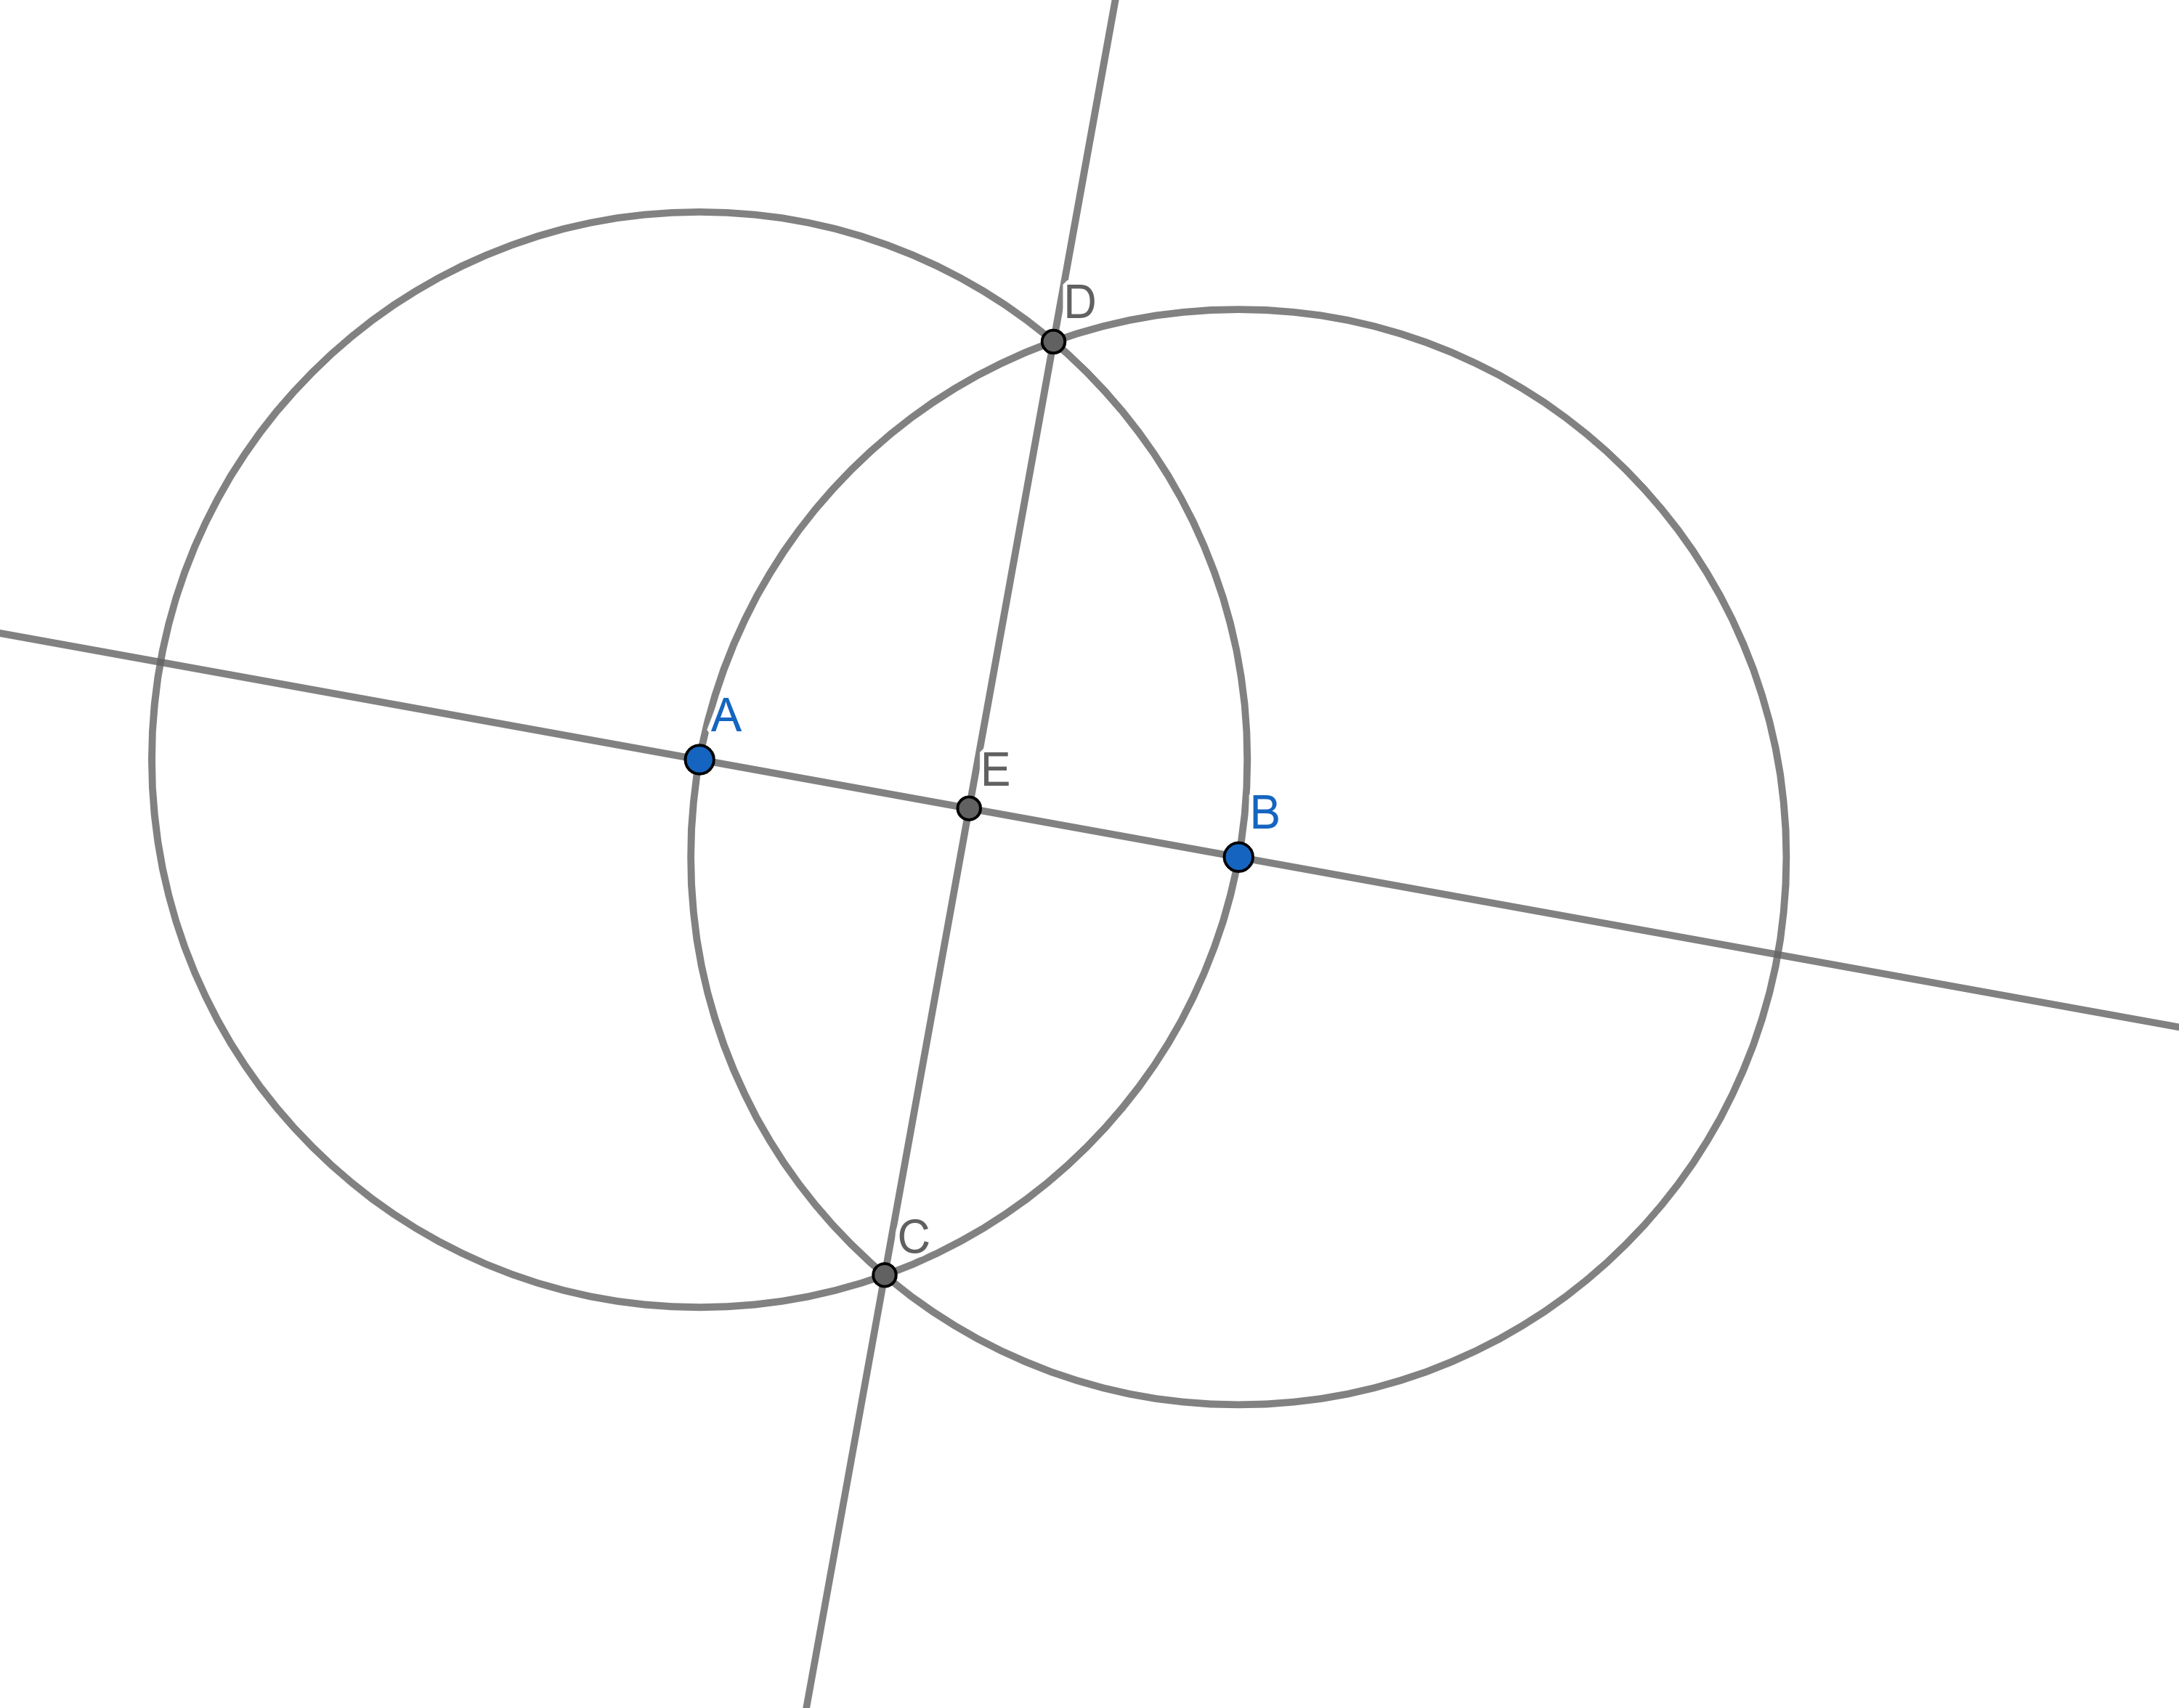
\includegraphics{geogebra-midpoint.png}}

Notice that the construction above also shows how to construct a line that is perpendicular to a given one, and how to construct an equilateral triangle.

When GeoGebra was first released the set of Geometry tools was very limited, but over time they expanded the toolkit -- after all, once you've figured out how to construct a perpendicular bisector, why not just let you click a single button to get one.  Still, some of the tools that are now available stretch the rules of Euclidean geometry.  For instance there is a proof that it's impossible to construct a regular heptagon (that would be a 7-sided polygon with all edge lengths and all angles equal), but there's a tool in GeoGebra that will let you construct a regular polygon with any number of sides that you desire.

In the lab, we're asking you to explore the notion of constructability, but many of the constructions can be accomplished with a single click if you find the right thing to click on.  Please restrict yourself to only using the tools that are ``allowed'' for each exercise.

 \clearpage
 \begin{worksheet}{15}{Geometric Constructions}{GeoGebra.png}
 \begin{enumerate}

\item Start GeoGebra, sign in, and change the mode from ``Graphing'' to ``Geometry''

\vfill

\item When you first enter the ``Geometry'' mode the tool panel will have a very limited number of options.  All but one of the things we'll need for the first task are here -- the additional tool is call ``Intersect'' and you'll need to fully expand the tool panel to find it.  Use points, lines, circles and the ability to construct points at the intersection of two curves to construct an equilateral triangle.

\vfill

\item Create a line and a point that's not on the line.  Can you use the basic tools (constructing lines and circles, finding intersections) to create a line that goes through the point, which is also perpendicular to the original line?

\vfill

\item Once you've completed the previous task, we're justified in letting you use the ``Perpendicular Line'' tool.  Using the basic tools plus ``Intersect'' and ``Perpendicular Line'' construct a square.

\vfill

\item Using the same tools, construct a right triangle where one leg is twice as long as the other.  If we say the short side is one unit long, how long is the hypotenuse of this triangle?

\vfill

\item There is a number you may have heard of called $\phi$ -- the golden proportion.  Its value is $\displaystyle \phi = \frac{1+\sqrt{5}}{2}$.
A golden rectangle is a rectangle whose side are in the golden proportion, so if you can construct a rectangle with sides $2$ and $1+\sqrt{5}$ you will have made a golden rectangle.  Referring to the previous problem, you should be able to do it!

\vfill

\item Let's finish up by exploring some properties of triangles.  Feel free to use any of the tools for these questions.
There are several ways to find a point that can be regarded as the ``center'' of a triangle.  Use Geogebra to construct all of the following:

\begin{enumerate}
	\item The line segments that go from a corner to the midpoint of the edge across from it.  There are three of these, which intersect in a point called the {\em mediant}.
	\item The line segments that are perpendicular to an edge and pass through the point across from the edge.  These intersect in a point called the {\em orthocenter}.
	\item The lines that bisect the angles at each vertex.  These intersect in a point called the {\em incenter}.
\end{enumerate}

\item Create a single triangle and construct the mediant, orthocenter and incenter.  Change the settings so that each type of ``middle'' is constructed with a different color.  Now move the corners around to see if

\begin{enumerate}
	\item it is possible to make all 3 centers coincide.
	\item it is possible to make two centers coincide while the 3rd is different.
\end{enumerate}

\end{enumerate}

 \end{worksheet}
 \clearpage

\section{Parabolas}

You may recall that parabolas are one of the conic sections we played with in lab 14.  As a conic section, a parabola is the intersection of a plane with a cone -- when the plane is parallel to the side of the cone.  There is an alternative way of defining a parabola, which doesn't require us to do anything in 3-d.  Working strictly in the 2-dimensional Euclidean plane we can define a parabola as ``the set of points that are equidistant to a point and a line.''

Let's unpack that definition a little.  There are two ingredients, a line and a point.  The line is called the {\em directrix} and the point is called the {\em focus} of the parabola.  If the focus happens to lie on the directrix we get a degenerate case: the parabola turns into a line.  (This degenerate situation can also be seen in the conic section version of things -- when the plane passes through the tip of the cone.)  To say that a point is equidistant to two things just means that the distance between the point and thing one is the same as the distance between the point and thing two.  Distance between a couple of points is straightforward, but how do we measure the distance between a point and a line?  Short answer: measure perpendicular to the line.

\centerline{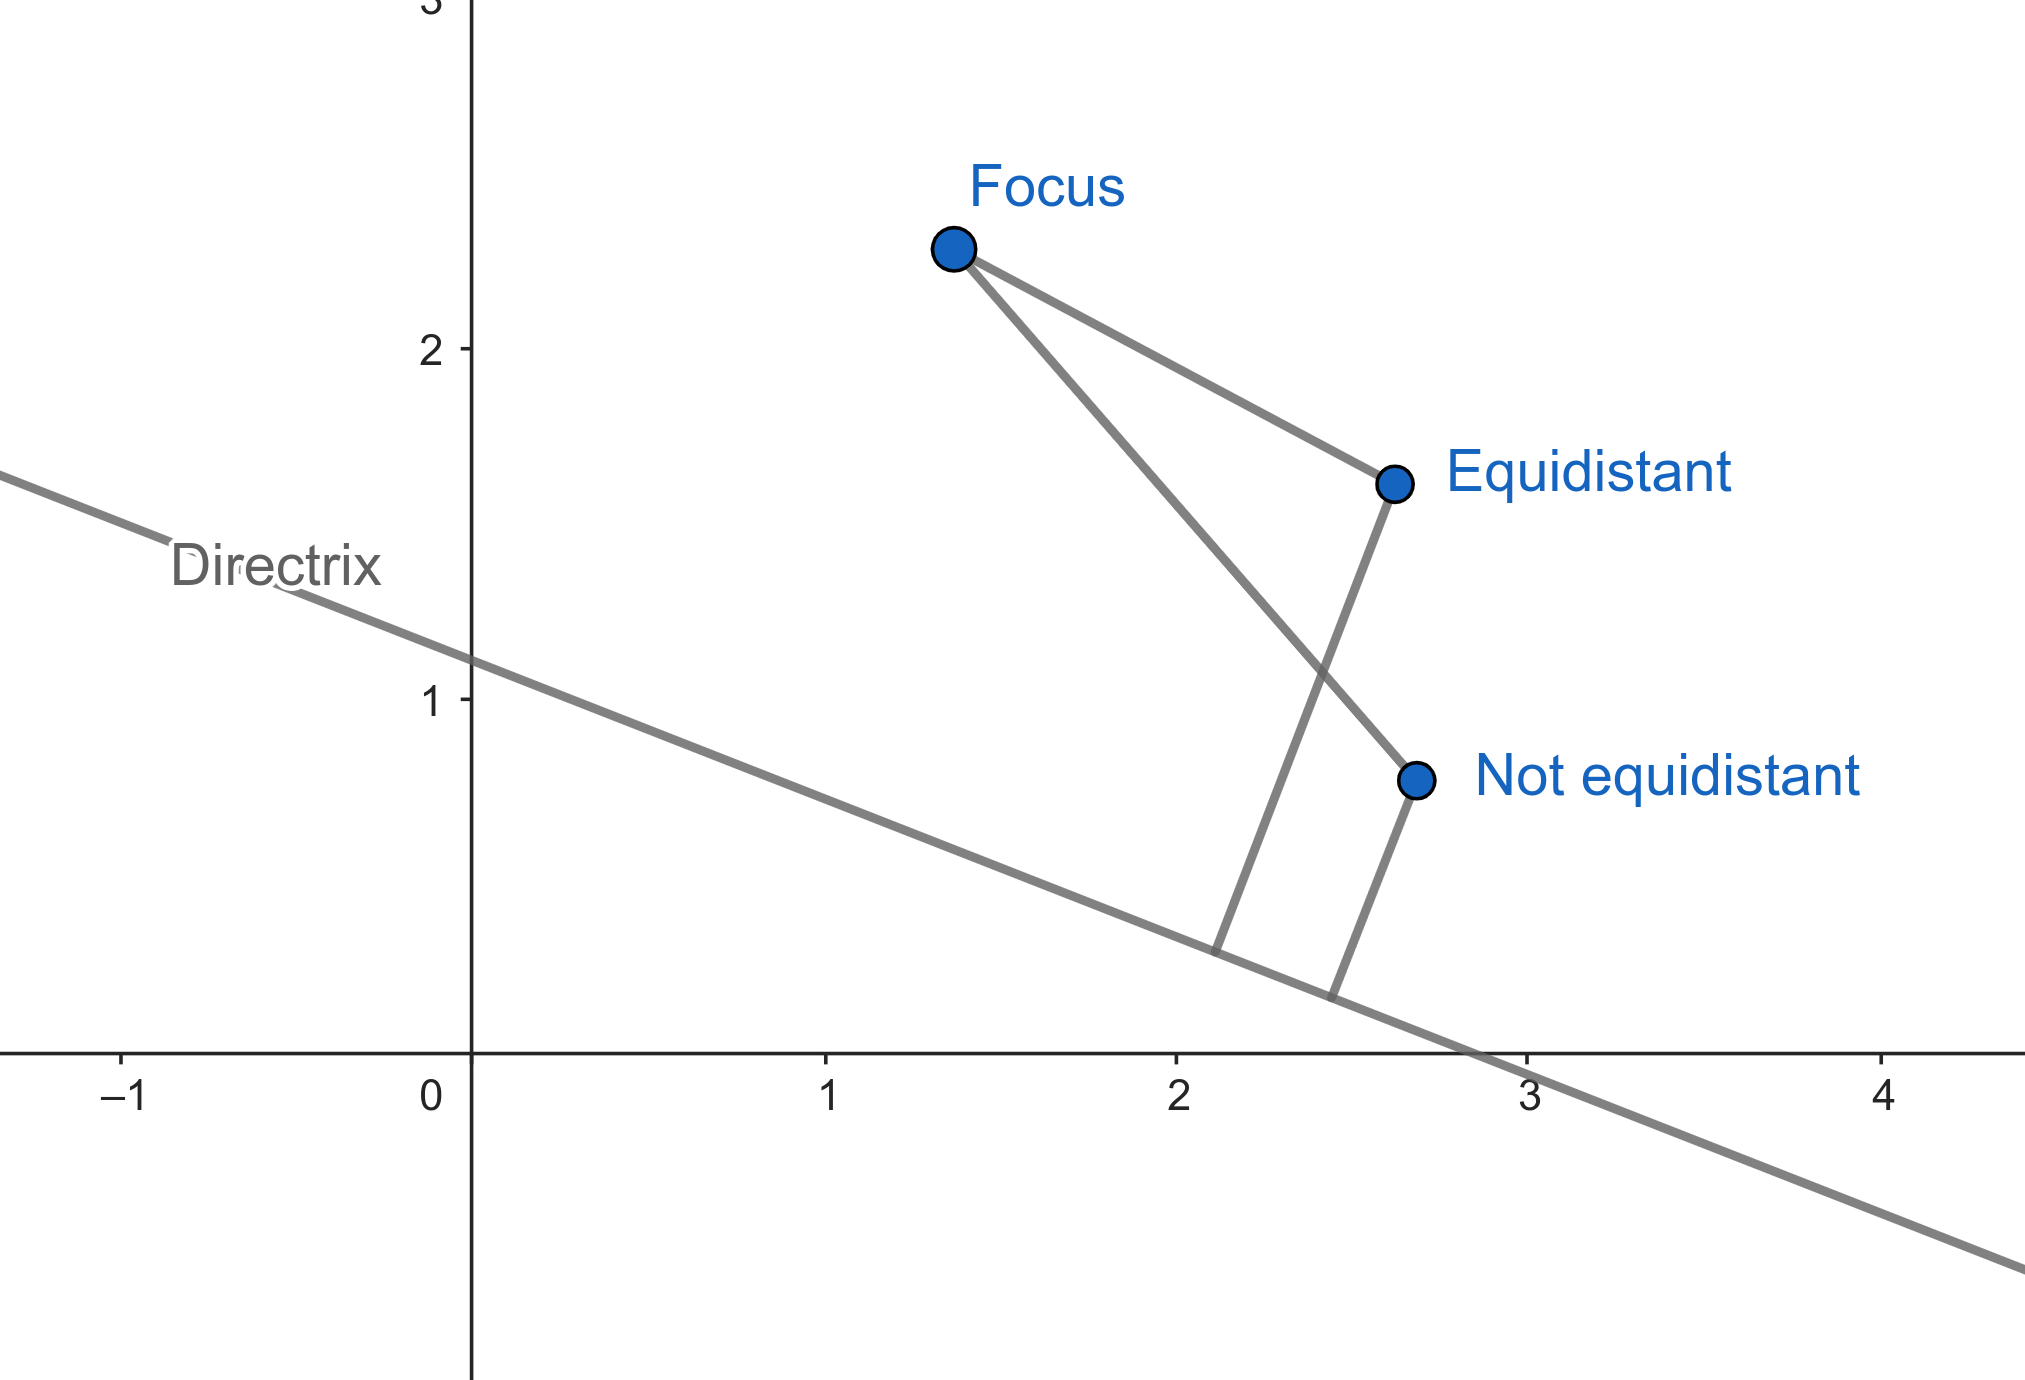
\includegraphics{focus-directrix.png}}

Only one of the points in the figure satisfies the condition of ``being equidistant between the focus and directrix'' so that one would be on the parabola, and the other would not.  Of course, there are many other points which satisfy this ``equidistant'' condition, and when we fill them all in we get our parabola.

\centerline{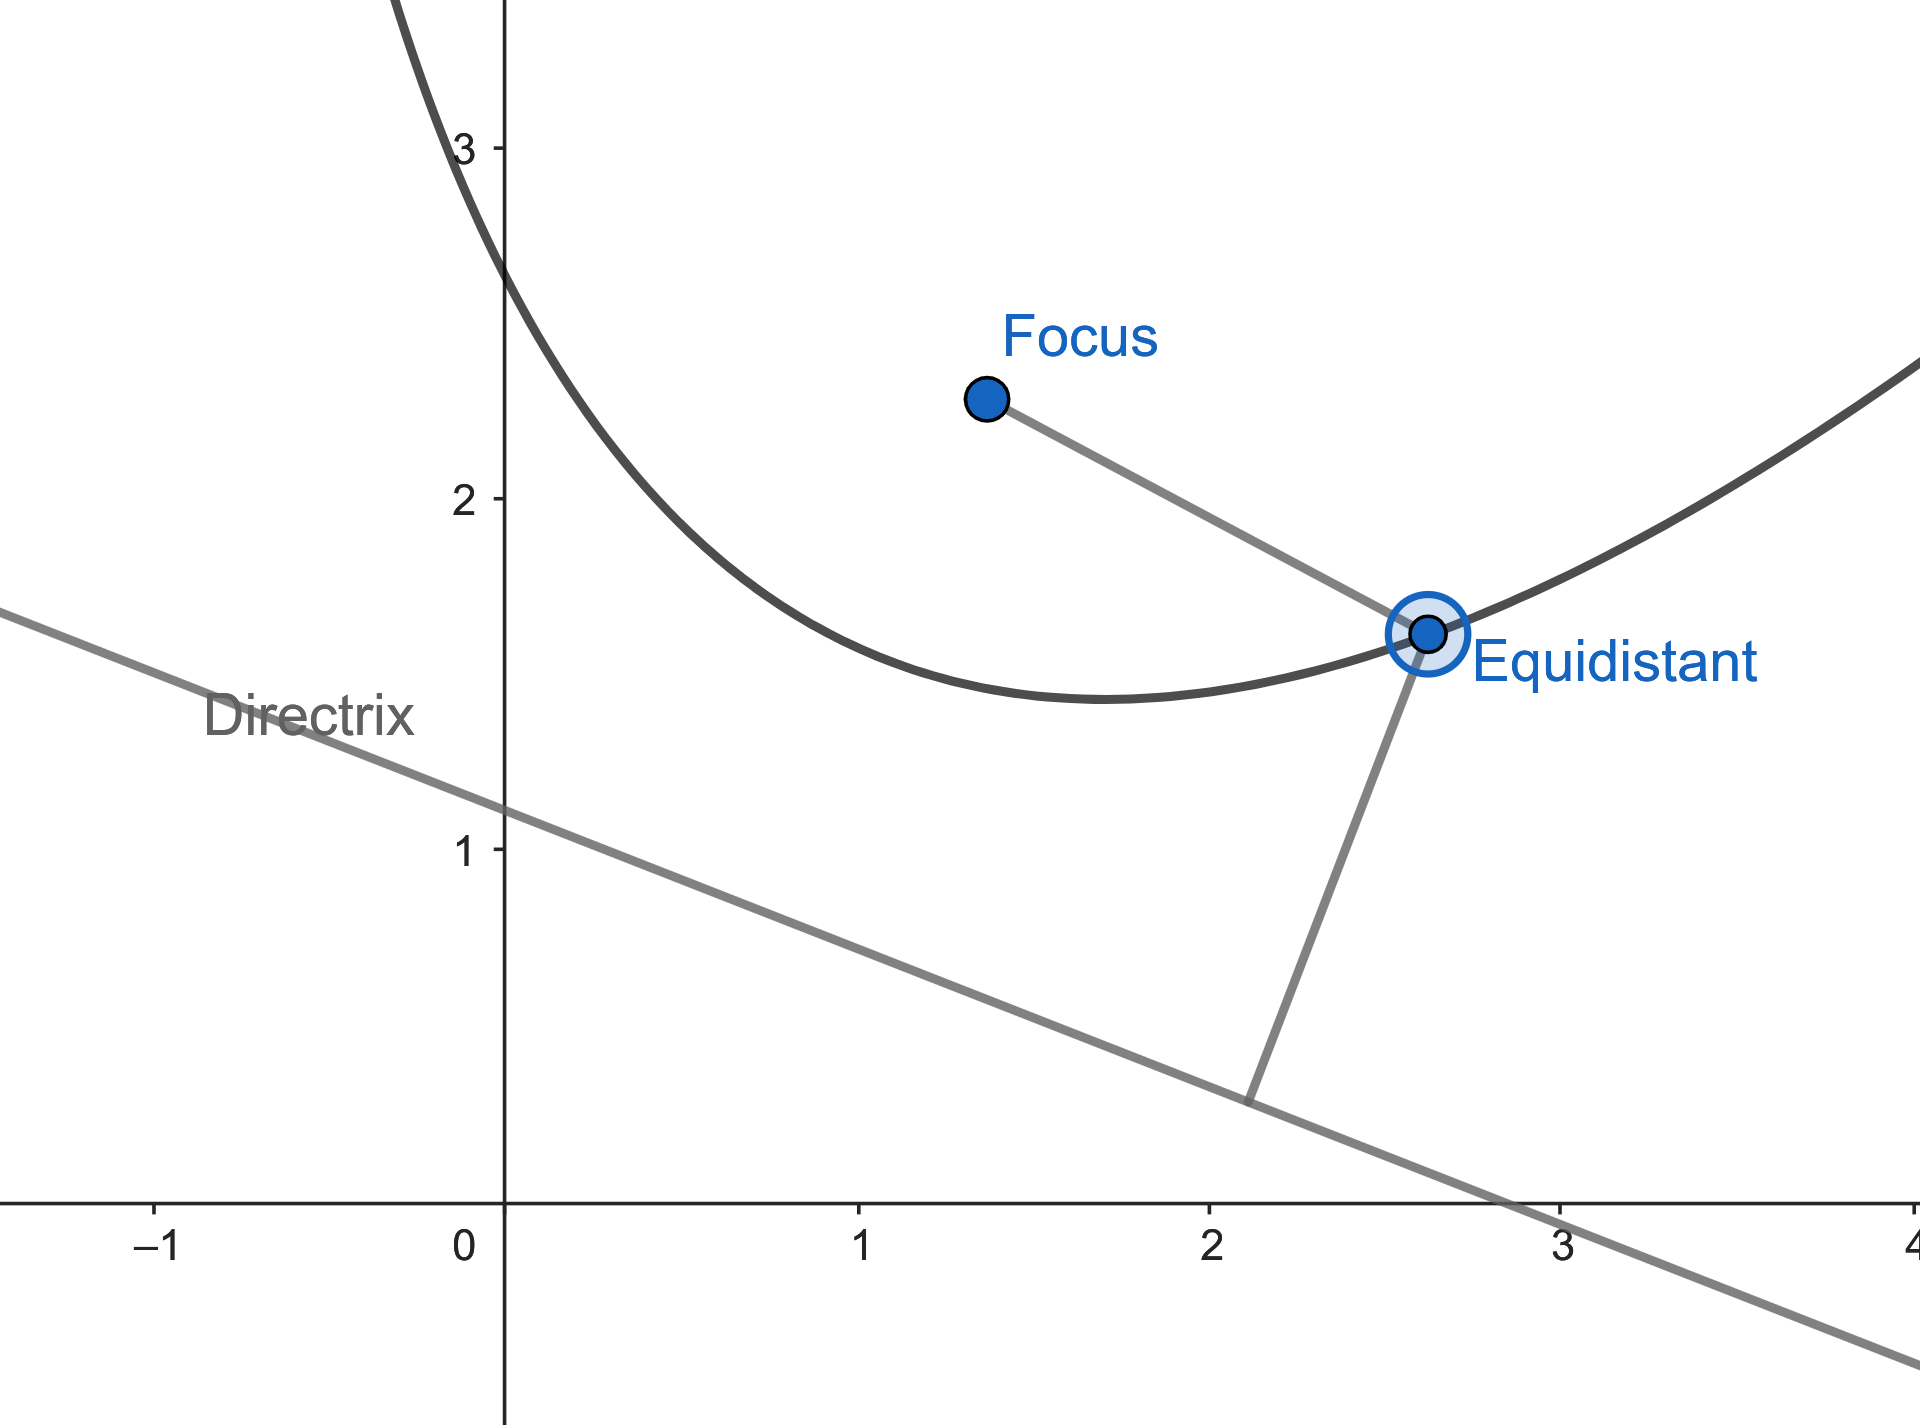
\includegraphics{parabola.png}}

In the lab for this section we'll explore this a bit more.

\clearpage
 \begin{worksheet}{16}{Parabolas}{GeoGebra.png}
 
\noindent In this lab, you will learn how to use GeoGebra to construct a geometric object and how to apply the distance definition of parabola to analyze your construction. Remember, \textbf{a parabola} is the set of points equidistant from a fixed point (the focus) and a fixed line (the directrix). 
\vspace{0.2 in}

In fact, you can create a parabola with nothing more than a sheet of wax (or plain) paper and a single point on the page! The video in this link will show you how one can fold paper to create a parabola: \url{https://www.youtube.com/watch?v=GdJlbNweSVY}. 

\vspace{0.2 in}

But, creasing your paper takes some work. Folding one or two sheets is fun, but what would happen if you wanted to continue testing many different locations for point A? You’d need to keep starting over with fresh paper, folding new sets of creases. Technology can streamline your work. With just one set of creases, you can drag the Focus point to new locations and watch the crease lines adjust themselves instantaneously!


\begin{enumerate}

\item Before trying this on the computer, try doing it with actual paper!

\vfill

\item Start GeoGebra, sign in, and put it in ``Geometry'' mode.

\vfill

\item Use the Line tool to draw a horizontal line near the bottom of the screen. This line AB represents the bottom edge of the paper (the directrix of the parabola).

\vfill

\item Draw a point C above the line, roughly centered between the left and right edges of the screen.	This point will be the focus of your parabola.

\vfill

\item Construct a point D anywhere on the horizontal line and construct the “crease” formed when point D is folded onto point C. There may be other options, but the ``perpendicular bisector tool'' would be a good choice.

\vfill

\item Drag point D along its line. If you constructed your crease line correctly, it should adjust to the new locations of point D.

\vfill

\newpage

\item Select the crease line and choose ``Show trace'' from the right-click menu.

\vfill

\item Drag point D along the horizontal line to create a collection of crease lines.

\vfill

\item To see other cases, you'll want to clear the traces.  Look in the drawing window settings (the gear in the upper right corner of the drawing area) and select ``Clear all Traces.''  Now try moving the focus (point C) to a different location.

\vfill

\item Again, drag point D to create another collection of crease lines.

\vfill 

\item There is a point that actually traces out the parabolas we've been looking at.  It lies at the intersection of the crease line and a line through D, perpendicular to the directrix.  Construct it!

\vfill

\item To create the graph of your parabola, without all the trace lines, check out the ``Locus'' tool.  It draws the path that a point, whose position is determined by something else, will move in.  The tool tip on this is not terribly clear - click the ``Locus'' tool, then the point whose path you want drawn (the locus point) and then the point that controls its motion (point D in this case).

\vfill

\item You can also create the graph of a parabola using the Algebra panel.  Just type \verb+y = x^2+, and you'll get the parabola most people think of when the hear the word ``parabola.''  Challenge: move the directrix and the focus around until you get a close match.

\vfill

\item Final Challenge: What do the think are the actual locations of the focus and the directrix for $y=x^2$?




\end{enumerate}

 \end{worksheet}
\clearpage

\section{More with GeoGebra}

The GeoGebra project started as a tool for doing Geometric constructions.  Over the years, many other capabilities have been added to it.

The selection box at the top/center of the GeoGebra window allows you to choose between several modes: Graphing, 3D Calculator, Geometry, CAS (Computer Algebra System) and Probability.  So far, we've looked mainly at the Geometry mode, but today we'll explore some of the others.

There is a mathematical area that works well as an arena for looking at the Graphing, 3D Calculator and CAS modes.  It's known as ``systems of linear equations.''

The simplest possible ``system'' would have a single equation and there would be only 1 variable too.  For example,

\[ 2x = 8. \]

That's obviously a little too simple!  

Here's a system where there are two variables and two equations:

\begin{align*} x + y &= 14 \\ 
 x - y &= 6 
 \end{align*}
 

That's a little more complicated, but you can probably find the answer by a little bit of ``guess and check.''  We're looking for two numbers that add up to 14 and which differ by 6.

Several years ago when you were first learning about linear equations you would have encountered several ``forms'' for the equation of a line

\begin{itemize}
	\item[slope-intercept form] \rule{0pt}{24pt} \rule{12pt}{0pt} $y = mx + b$
	\item[point slope form] \rule{0pt}{24pt} \rule{12pt}{0pt} $y = m(x - h) + k$
	\item[standard form] \rule{0pt}{24pt} \rule{12pt}{0pt} $ax + by = c$
\end{itemize}

At the time you may have thought that standard form should really be the $y=mx+b$ thing, and that the actual standard form was rather poorly named.  It's at this point (while looking at systems of linear equations) that we see what makes standard form so useful.  One thing that's worth pointing out: in the other two forms, one of the variables is singled out (both of them are solved for $y$), standard form is more egalitarian, neither variable is prefered over the other.

\clearpage
 \begin{worksheet}{17}{More with Geogebra}{GeoGebra.png}
 

\begin{enumerate}

\item Find two numbers that have a sum of 26 and which differ by 8.

\vfill

\item Start GeoGebra, sign in, and put it in ``Graphing'' mode. In the input cells we're going to enter two formulas.  The first is $x+y=26$ and the second is $x-y=8$.
Describe the shapes that are created in words.  What is the significance of the point $(17,9)$ in this picture?

\vfill

\item Consider the pair of linear equations

\[ y = 3x+ 5 \quad \mbox{and} \quad y=-x+3 \]

Graph both of them in the ``Graphing'' window, and find their point of intersection.  What is the significance of this point?

\vfill

\item Here are a couple of linear equations in standard form.

 \[ 3x + 2y = 7 \quad \mbox{and} \quad x - 2y = 5 \]

 Verify that you can get their graphs in GeoGebra without having to first put them in slope-intercept form.  (I.e. GeoGebra is perfectly happy dealing with lines that are in standard form.)  What values of $x$ and $y$ make both of these equations true simultaneously?

 \vfill

\item We've seen that when we graph a linear equation in two variables we get a line in the plane, and when we graph two such things we typically can find a point where they intersect - which is a simultaneous solution to the two equations.  What does this all look like if there are more than two variables?
Switch to the ``3D Calculator'' mode and create a graph of $x+y+z=5$.  Geometrically, what is it?

\vfill

\item Adding a couple of more equations, we get a system of 3 equations in 3 variables:

\begin{align*}
x + y + z &= 5\\
x - y \phantom{ + zz } &= 1\\
x + y - z &= -1
\end{align*}

Create 3D graphs of all three and verify that the point $(1,0,4)$ is the intersection of the 3 planes.

\vfill

\item Sadly, there is no 4D mode for GeoGebra, and to be honest, even in 3D finding a point at the intersection of three planes isn't very easy!  Certainly not as easy as the 2D version of things: finding the intersection of two lines.  This is where the CAS mode comes to the rescue.  We're going to use the CAS mode to work with {\em matrices}.  Matrices are simply tables of numbers -- in the current setting a good way to think of them is as a system of equations with all the decorations removed.  We don't need to write the variables (we always write them in the same order anyway) we just record the coefficients of them.  There's not even a reason to write the $=$ signs - they always come right before the last number in a row (which is whatever is on the right-hand side of the equation).

Here's a very simple system of equations:

\begin{align*}
x + y &= 14\\
x - y &= 6\\
\end{align*}

This is how it looks as a matrix:

\[ \left( \begin{array}{ccc} 1 & 1 & 14 \\ 1 & -1 & 6 \end{array} \right) \]

To enter a matrix into GeoGebra we use nested French braces.

Switch to ``CAS'' mode and enter the following:

\verb+ A = {{1,1,14},{1,-1,6}}+

Press ``Enter'' and it should display a pretty matrix named $A$.

\vfill

\item There is a command in GeoGebra's CAS which is too long to type.  Try typing ``Red'' and then click on the suggestion that pops up.  You want to run a command that looks like

\verb+ReducedRowEchelonForm(A)+

We already know that $x=10$, $y=4$ is the solution to that system.  (If not, take a second to work that out in your head.)  Can you see this solution in the output of that last command?

\vspace{.7in}

\item Final Challenge: Convert the system of linear equations
\begin{align*}
x + y + z &= 5\\
x - y \phantom{ + zz } &= 1\\
x + y - z &= -1
\end{align*}

into a matrix and use \verb+ReducedRowEchelonForm()+ to find its solution.

\vfill

\end{enumerate}

 \end{worksheet}
\clearpage

\section{Projects}

\subsection{A pentagon}

There is a way to create any regular pentagon in GeoGebra.  The challenge of this project is to use the basic Greek geometry tools to construct a regular pentagon -- but do it in GeoGebra.

\subsection{Tilings}

Among the works of the famous Dutch artist M.C. Escher, there are \href{https://mcescher.com/gallery/symmetry/}{many} that illustrate tilings of the plane with recognizable figures.  Such tilings must of necessity involve some of the basic transformations that are found in the GeoGebra toolkit.

\begin{enumerate} 
	\item translations
	\item rotations
	\item reflections
	\item glide-reflections (a combination of translation and reflection)
\end{enumerate}

Use GeoGebra to create an Escher-like tesselation of the plane.  A good intro about how to make a tesselation is \url{https://www.youtube.com/watch?v=Ggk6n-RX4OQ}.

\subsection{Quadric surfaces}

In 2-D we talked about the conic sections.  It turns out that these are also all the types of curves which are the graphs of quadratic relations in two variables.
Use the 3D Calculator in Geobegra to find all of the 3D quadratic surfaces (although, for unknown reasons, in this context, people say ``quadric'' rather than ``quadratic'').
Some judicious Googling might help.

% 
\chapter{Statistics}


\section{R}
\label{sec:r}

\subsection{Getting access to R}

\subsubsection{R in your Browser}

Log into your CoCalc account and create a new sage worksheet. There is something called ``cell magic'' that changes the nature of a cell so that it ``understands'' other languages besides sage.  For instance, typing \verb+%md+ on the first line of a cell makes that cell a markdown cell.  Typing \verb+%r+ on the first line of a cell makes that cell an R cell.

It's easy to forget to put in the cell magic, which leads to some hilarious (but disconcerting) error messages.  Fortunately, there's a way to set the cell magic globally.
If you put \verb+%default_mode r+ in the first line of the first cell of a worksheet (and execute it!) then all of the cells will be treated as containing R code.

% ~~~~~~~~~~~
\subsubsection{Downloading R and RStudio}

There's no need to do this for today's lab, but if you want to get R running on your own machine\dots

To download R to your computer, you need to download two pieces of software
\begin{enumerate}
\item R, which is like the engine underneath the hood
\item RStudio, which is the controls and the software you'll actually work with.
\end{enumerate}

To begin your download of R, click on the following link

\begin{center}
  \href{http://lib.stat.cmu.edu/R/CRAN/}{http://lib.stat.cmu.edu/R/CRAN/}
\end{center}

Then select the link corresponding to your computer type.

Move forward as if downloading any other program. Once you download R, you still need to download RStudio.

% ~~~~~~~~~~~~~~~~~~~~~~~~~~~~~~~~
\subsubsection{Downloading RStudio}

To begin downloading RStudio, click on the following link

\begin{center}
\href{https://www.rstudio.com/products/rstudio/download/}{https://www.rstudio.com/products/rstudio/download/}
\end{center}

Select the ``Download RStudio Desktop'' button


Then select the download link corresponding with your operating system.


\subsection{Variables}
\label{sec:r_variables}

In the context of R, the term \textbf{variable} is not an unknown
quantity to be determined, as in ``Solve for $x$ in $3x-5=10$'' It
\textbf{is} a nickname, given for convenience.  We will know exactly
what it is, because we define it.  

A slight oddity of the R language is that we don't use an equals sign ($=$) to assign a nickname, instead we type \verb+<-+ which is supposed to look like a left-pointing arrow.

Sometimes, we like to choose a short variable name that is simple to type
  
\begin{example}
  \begin{rcode}    
    a <- 5 # assign the name 'a' to the value '5'
    3*a
    5*a^2+5
    
    b <- 2*a-6
    b
    
    3*a^b-2
  \end{rcode}
\end{example}

Othertimes, it's best to use a variable name that is descriptive so
when we read our code later, we understand what it is doing

\begin{example}[Convert kg to lb's]
  \begin{rcode}    
    weight_kg <- 50 # assign name weight_kg to the number 50
    weight_lb <- 2.2*weight_kg # assign convert weight_kg and assign new name
    weight_lb # print the value of weight_lb
  \end{rcode}
  \textbf{Important:} can't use spaces in variable names, use underscore instead.
\end{example}
  
% ~~~~~~~~~~~~~~~~~~~~~~~~~~~~~~~~~~~~
\subsection{Functions}
\label{sec:r_functions}

We'll learn a bunch of \define{functions} in R.  

\begin{example}[Absolute Value Function]
  The absolute value function is written like ``abs()''.  Place the
  value you want to take the absolute value of into the parenthasis.
  \begin{rcode}
    abs(4) # absolute value of 4
    abs(-3) # absolute value of -3
    
    x <- -3*5 + 2
    abs(x)
    abs(-3*5+2) # same as abs(x)

    abs(y) # notice the error because we haven't told R what 'y' is
  \end{rcode}    
\end{example}

\begin{example}[Rounding function]
  A common function we'll want to use to rounding numbers.  There is
  a function to do this for us.  Using this function is better than
  doing it yourself.
  \begin{rcode}
    number <- 4.3134314512351
    round(number) # round to nearest whole number
    round(number, 2) # round to 2 decimal places
    round(number, 4) # round to 4 decimal places
  \end{rcode}    
\end{example}

It is incredibly common to forget exactly how a function works, or
maybe you're getting an error that you can't quite crack. There are
two ways of getting help.

\begin{enumerate}
\item Google.  If you can't recall how the \texttt{round()} function
  works, google ``round function R''
\item Help within R itself.  There is an R function called \texttt{help()} -- put whatever R command you're interested in in the parentheses.
\item If you're running RStudio, go to the lower right window, click the
  'help' tab, and search for your function.
\end{enumerate}

\subsection{Exercises}

\begin{q}
  What R code is used to compute the following expressions?
  \begin{enumerate}
  \item Subtract 10 from 2 
  \item Multiply 3 by 5
  \item Divide 9 by 2
  \item From 5, subtract 3 times 2
  \item Double the difference of 5 and 3
  \item Four squared
  \item Divide 8 by 2 squared
  \end{enumerate}
\end{q} 

% ~~

\begin{q}
  Consider the following R code.

\begin{rcode}
mass_kg <- 2.62 
mass_g <- mass_kg * 1000 
mass_g 
\end{rcode}

\begin{enumerate}
\item Explain in plain language what the following three line program
  does, i.e. state what each line does and what the meaning of the
  output of the program is
\item  Run the program. (Hit enter after each line break.) What is its output?  
\item  Modify this code so that it converts the inital mass to pounds (there are 2.2
  pounds in a kilogram) and print the resulting mass.  Run this
  program.
\end{enumerate} 
\end{q} 

% ~~

\begin{q} 
  Run \texttt{help(abs)} in R. What happens?  Familiarize yourself
  with the built-in functions \texttt{abs()}, \texttt{round()},
  \texttt{sqrt()} by running this ``help function'' on \texttt{round}
  and \texttt{sqrt}. Use these built-in functions to create R code to
  accomplish the following:

  \begin{enumerate}
  \item The absolute value of -15.5.   
  \item 4.483847 rounded to one decimal place. 
  \item Assign the value of the square root of 2.6 to a variable. Then
    round the variable you’ve created to 2 decimal places and assign
    it to another variable. Print out the rounded value.
  \end{enumerate} 
\end{q}

% ~~

\begin{q}
  The following code estimates the total net primary productivity
  (NPP) per day for two sites. It does this by multiplying the grams
  of carbon produced in a single square meter per day by the total
  area of the site. It then prints the daily NPP for each site.

\begin{rcode}
site1_g_carbon_m2_day <- 5 
site2_g_carbon_m2_day <- 2.3 
site1_area_m2 <- 200 
site2_area_m2 <- 450 
site1_npp_day <- site1_g_carbon_m2_day * site1_area_m2 
site2_npp_day <- site2_g_carbon_m2_day * site2_area_m2 
site1_npp_day 
site2_npp_day 
\end{rcode}

\begin{enumerate}
\item Explain what each line does. You can refer to each line number, e.g. ``Line 1 does so and so''. 
\item Run the program using an RScript (upper left window, highlight
  everything, then click 'Run'). What is the output of the program?
\item Continuing the above code, write a line of code for each of the
  following items
  \begin{enumerate}
  \item The sum of the total daily NPP for the two sites combined.  
  \item The difference between the daily NPP for the two sites. We
    only want an absolute difference, so use abs() function to make
    sure the number is positive.  
  \item The total NPP over a year for the two sites combined (the sum
    of the total daily NPP values multiplied by 365).
  \end{enumerate}  
\end{enumerate}

\end{q} 

% ==================================
\section{Vectors in R}

One of the most fundamental objects we work with in R is known as a vector.  Think of it like a list of values. Often it may come as a column from a spreadsheet.  R gives us ways to perform different mathematical tasks with these vectors.  In this topic, most of the vectors will not contain too many items, so we'll learn what R can do in situations when we could just as easily do it by hand or a basic calculator.  But the real benefit of R comes into play when working with much larger datasets.

By the end of the section, you'll know 
\begin{enumerate}
\item How to create a vector and provide it a variable name
\item Modify a vector by adding new items to it
\item Perform algebra with vectors
\item Various functions that tell us certain features of vectors, like how long it it, it's largest/smallest value, the sum of all the entries, the mean of the entries
\item How to extract entries with certain properties, e.g. the 23 entree, or the entries larger than 5, etc.  
\end{enumerate}

% ~~~~~~~~~~~~~~~~~~~~~~~~
\subsection{Motivation}

In many statistical scenarios, we'll work with databases. Think of these like an Excel
spreadsheet. We'll get to working with those in R soon enough, for 
now, here's a simple one we're familiar with, a grade sheet
\begin{center}
  \begin{tabular}{cccc}
    \textbf{Student} & \textbf{HW1} & \textbf{HW2} & \textbf{Exam1} \\
    \hline\hline
    Joe              & 35 & 45 & 84 \\
    Jen              & 42 & 48 & 91 \\
    Jes              & 37 & 42 & 85 \\
    Jon              & 32 & 40 & 78 \\
    $\vdots$ & $\vdots$ & $\vdots$ & $\vdots$ \\
  \end{tabular}
\end{center}

A common task is to want to separate out a column, say ``HW1'', and
work with that because maybe you want to
\begin{itemize}
\item add 5 points to every score because a question wasn't fair
\item divide by the total number of possible points to get a percentage score
\item add columns together to get a total HW grade,
\item etc
\end{itemize}

A column in a database like this is simply a vector.
  
% ~~~~~~~~~~~~~~~~~~~~~~~~~~~~~~~~~~~~
\subsection{Defining Vectors}

A vector is a list of either numbers or of words. There is an
R-function to create a \define{vector},

\begin{rcode}
# generic column function
c()

# list with numbers 1,2,3,4
c(1,2,3,4)

# a list of names, note the quotes
c("jim", "james", "jimmie") 
\end{rcode}

Notice those lies that start with a `\#`?  Those are what computer programmers call \define{comments}.  That hash character tells the computer to ignore anything written behind it. This gives the human reading the code a chance to make notes right inside the code in a way that does not cause the computer to make an error.

We just filled a vector with names surrounded by quotations

\begin{rcode}
  c("jim", "james", "jimmie")
\end{rcode}

This ensures that the vector is filled with what are called
\define{strings}, which is a computer science way of saying a sequence
of letters or numbers. If you didn't include the quotations, the
computer reads them as variables. If you never defined a variable
named \texttt{jim}, or \texttt{james}, or \texttt{jimmie}, then you'd
get an error.

\begin{rcode}
  c(jim, james, jimmie) # should produce an error
\end{rcode}

But if you define these variables, then your vector will be filled
with those values.

\begin{rcode}
  c("x", "y", "z") # vector with the letters in each position
  c(x,y,z) # error b/c we never defined variables x,y,z

  # let's define x,y,z as variables 
  x <- 5 
  y <- 12 
  z <- 13 
  c(x,y,z) #no longer an error

    c("x", "y", "z") # still a vector with strings
  \end{rcode}
    
We can name columns to more easily refer to them

\begin{rcode}
  column_1 <- c(5,3,5,7,25,234)
  column_2 <- c("naomi", "wilshi")
  primes <- c(2,3,5,7,11)
  evens <- c(2,4,6,8,10,12,14,16)
\end{rcode}

Then to view them, compile just the name

\begin{rcode}
  column_1 
  column_2 
  primes 
  evens 
\end{rcode}

Suppose you're studying mice, you did an experiment with five mice and
you weighed each. So you created two vectors

\begin{rcode}
  names <- c("mouse_01", "mouse_02", "mouse_03", "mouse_04", "mouse_05")
  weight_g <- c(50,60,65,82,67)
\end{rcode}

If we continued the experiment and want to add another mouse and its
weight to our vector, we can do so by putting our previous vector
names into a new vector and name that.

\begin{rcode}
  names <- c(names, "mouse_06") # note variable in first spot, string in second
  weight_g <- c(weight_g,39)
  
  # print those
  names
  weight_g
\end{rcode} 

Note how these overrode the orginal columns \texttt{names} and \texttt{weight\_g}.  So if you are worried about making a mistake, it's a good practice to give the updated vectors a new name

\begin{rcode}
  # original vectors
  names <- c("mouse_01", "mouse_02", "mouse_03", "mouse_04", "mouse_05")
  weight_g <- c(50,60,65,82,67)
  
  # update them with new mouse info    
  names_v2 <- c(names, "mouse_06") # note variable in first spot, string in second
  weight_g_v2 <- c(weight_g,39)
  
  # now we still have the original
  names
  weight_g
\end{rcode} 

% ~~~~~~~~~~~~~~~~~~~~~~~~~~~~~~~~~~~~
\section{Vector Arithmetic}

In this section, we are going to learn how to add, divide, multiply, and divide. The difference between this and typical algebra is that, typically, you do them to a pair of numbers.  Here, we're going to (1) do the algebra with a number and a vector, and also (2) with two vectors.
  
The the following. Give a variable name to any vector with only
numbers (i.e. no strings) of any length.  Then to that vector add a
number to it, subtract a number from it, multiply it by a number,
divide it, raise it to some power.


Now try this. Give two variable names to two vectors whose elements
are all numbers (i.e. no strings). The vectors should be be the same
length. Then add them together, subtract them, multiply them together,
and raise one to the power of the other.

Now repeat this, except make one vector have length 3 and the other of
length 4. Repeat again except make one vector length 2 and the other
length 4.  Note what happens.

% ~~~~~~~~~~~~~~~~~~~~~~~~~~~~~~~~~
\subsection{Functions on Vectors}

Just like you can plug numbers into R-functions, there are certain
R-functions that we can plug vectors into.
  
Recall that vectors, for us, will typically be filled with data. Perhaps its a column from a database, e.g. a gradebook. Here are some common things we'd want to be able to do with it.
  
\begin{example}
  \begin{rcode}
    hw1_grades <-  c(51,21,35,15,35,15,23,65,15,35,13,54,2
    6,35,12,45,12,35,58,54,43,49,47,45,42,41,43,46,48,54,42,48,47)
    
    length(hw1_grades) # returns how many items are in the list
    max(hw1_grades) # returns the max grade
    min(hw1_grades) # returns the min grade
    sum(hw1_grades) # adds all the grades together
    mean(hw1_grades) # returns the mean grade
    summary(hw1_grades) # a convenient way to get a lot of information about how the grades are distributed
  \end{rcode}
\end{example}
  
% ~~~~~~~~~~~~~~~~~~~~~~~~~~~~~~~
\section{Subsetting Vectors}

Another important construction we'd like to be able to perform on a
vector is to look at certain parts of the vector. For example, maybe
we want to see just the 14th entry, or we want all the entrees above
10, or that are not 0.  This is called \emph{subsetting vectors}
because we are trying to extract a subset of the entrees in our vector
  
Here are various ways to get at some important information contained
within a vector.
  
\begin{rcode}
  # create an arbitrary vector
  x <- c(1,5,4,8,6,4,5,3,1,2,4,9,8,7,4,6,5,3,8,1,2,5,3,6,1,2,5,3)
  
  # to see just the 6th entry, replace 6 with any entry
  x[6]
  
  # to see the 3rd, 6th, 10th entry. Note the column function used to return multiply entrees
  x[c(3,6,10)]
  
  # to see all the entrees strictly greater than 5
  x[x > 5]
  
  # to see all entrees less than or equal to 7
  x[ x <= 7]
  
  # to see all entress that are not equal to 4
  x[ x != 4 ]
  
  # combine multiple properties with & (and) and | (or)
  x[ x>5 & x<=7] # returns 5<x<=7, we do need to use the & here
  x[ x < 3 | x >=8] # returns x str. less than 3 or at least 8    
\end{rcode}

% ~~~~~~~~~~~~~~~~~~~~~~~~~~
\subsection{Exercises}

\begin{q}
  Create a variable (any name you like) from the following vector
  (copy and paste, but make sure it's all on one line):

\begin{rcode}
  c(35,16,64,35,43,25,95,12,62,43,27,81,32,
  46,25,29,93,105,56,68,48,72,83,72,42,29,12,61,
  54,82,53,19,8,68,1,0,29,14,82,86,94,62,52,18,68,75,84)
\end{rcode}

  Using R, what command will print out the values that are
  \begin{enumerate}
  \item greater than 30
  \item not equal to 82
  \item between 45 and 75.
  \end{enumerate} 
\end{q} 

% ~~

\begin{q}
  The number of birds banded at a series of sampling sites has been
  counted by your field crew and entered into the following
  vector. Counts are entered in order and sites are numbered starting
  at one. Cut and paste the vector into your assignment and then
  answer the following questions by printing them to the screen (again
  be certain everything is on the same line). Some
  R functions that will come in handy include \texttt{length(), max(), min(),
  sum()}, and \texttt{mean()}.

\begin{rcode}
number_of_birds <- c(28, 32, 1, 0, 10, 22, 30, 19, 145, 27,36, 25, 9, 38, 21, 12, 122, 87, 36, 3, 0, 5, 55, 62, 98, 32,900, 33, 14, 39, 56, 81, 29, 38, 1, 0, 143, 37, 98, 77, 92, 83, 34, 98, 40, 45, 51, 17, 22, 37, 48, 38, 91, 73, 54, 46, 102, 273, 600, 10, 11)
\end{rcode}

What R command will give the answer the questions?
  \begin{enumerate}
  \item How many sites are there?   
  \item How many birds were counted at site 42?   
  \item What is the total number of birds counted across all of the
    sites?   
  \item What is the smallest number of birds counted?   
  \item What is the largest number of birds counted?    
  \item What is the mean number of birds seen at a site?   
  \end{enumerate} 
\end{q} 

% ~~

\begin{q}
  You have data on the length, width, and height of 10 individuals of
  the yew Taxus baccata (a type of shrub) stored in the following vectors:

\begin{rcode}
length <- c(2.2, 2.1, 2.7, 3.0, 3.1, 2.5, 1.9, 1.1, 3.5, 2.9)
width <- c(1.3, 2.2, 1.5, 4.5, 3.1, 1.7, 1.8, 0.5, 2.0, 2.7)
height <- c(9.6, 7.6, 2.2, 1.5, 4.0, 3.0, 4.5, 2.3, 7.5, 3.2)
\end{rcode}

  What R command will provide the following?
  \begin{enumerate}
  \item The volume of each shrub (i.e., the length times the width
    times the height). storing this in a variable will make some of
    the next problems easier
  \item The total volume of all of the shrubs.
  \item A vector of the height of shrubs with lengths greater than
    2.5.
  \item A vector of the height of shrubs with heights greater than 5.
  \item A vector of the heights of the first 5 shrubs.
  \item A vector of the volumes of the first 3 shrubs.
  \end{enumerate}  
\end{q}


%\section{spreadsheets}
%\label{sec:s}


\chapter{Symbolic Computer Algebra}

\section{Computations using computer algebra}

A \textit{computer algebra system} (or \textit{CAS}, for short) is software
that is able to perform algebraic procedures similar to what you would
normally do ``by hand.'' There are several popular CAS used in mathematics,
with the most common being Mathematica, Sage, and Maple. We will
be using Sage, as it is available as free open-source software, and it has been
largely developed by mathematicians, integrating many specialized packages
used by casual and professional mathematics researchers. Much of it
uses Python, so if you have any knowledge of coding in Python, you will find
Sage to be familiar; but fear not if you do not have any prior experience,
as the purpose of this lesson is to get the hang of the basics!

Sage can be installed on your computer or run from the CoCalc servers
if you create a (free) account. For now, we will use a lightweight version of Sage
that can be run on a webpage without any installation or other hassles.
 Go to \url{https://sagecell.sagemath.org/}.

You can enter basic Sage commands into the textbox on that page and
click ``Evaluate'' to get the output. We will begin by testing out some basic
arithmetic operations.

\clearpage
\begin{worksheet}{6}{Sage Cell Server}{sage.png}
Go to \url{https://sagecell.sagemath.org/}.

You can enter basic Sage commands into the textbox on the page and
click ``Evaluate'' to get the output.  To get started let's use sage like a fancy calculator.  The operands for sum, difference, multiplication, and division are \verb% +, -, *, / %.

Try the following operations:

\begin{enumerate}

\item Try the following operations:
\begin{enumerate}
	\item \verb% 1 + 2 + 3 %
	\item \verb% 42 - 23 %
	\item \verb% 1331 * 11 %
	\item \verb% 144 / 9 %
\end{enumerate}

    \item That's pretty standard stuff, you could more easily do those on your phone\dots  But, can your phone calculate 200 digits of $\pi$ in the blink of an eye?  Try this:

\begin{codeblock}
\begin{verbatim}
n(pi, digits=200)
\end{verbatim}
\end{codeblock}

    \item You may have noticed that the previous question's answers were all whole numbers, but this last one was a decimal.  We've been holding out on you a bit -- sage does {\em exact} computations.  Unless you ask it for a numerical approximation (which is what the 
    {\tt n( )} function was all about) it will give answers that are 100\% precise -- but sometimes that doesn't seem very helpful!  

    \noindent Try evaluating these:
    \begin{enumerate}
		\item \verb% pi %
		\item \verb% sqrt(2) %
		\item \verb% 7/3 %
    \end{enumerate}

    \item Sage and its brethren are Symbolic Computer Algebra Systems.  The reason it just parrots back the question to you has to do with the ``Symbolic'' part of that.  For example, the \verb+sqrt(2)+ thing above is regarded by Sage as a symbolic entity.  It is a full and precise representation of the number we write as $\sqrt{2}$.  It isn't some lame 4 or 10 or 100 digit {\em approximation} of $\sqrt{2}$. It is the real deal.  Let's see what happens when we raise \verb+sqrt(2)+ to various powers (you can use either \verb+^+ or \verb+**+ for exponentiation in sage).

	\noindent Try evaluating these:
    \begin{enumerate}
		\item \verb% sqrt(2) ^ 2 %
		\item \verb% sqrt(2) ^ 4 %
		\item \verb% sqrt(2) ^ 7 %
    \end{enumerate}

    \noindent Was the answer to that last one suprising?  Or does it make sense in retrospect?

    \item Much of the power of Computer Algebra comes from the same feature that makes regular Algebra useful -- variables.

    \noindent There are two kinds that we need to distinguish: computer variables and mathematical variables.  Computer variables are pretty easy, you can just make up whatever name you want and then start using it.  For example:

\begin{codeblock}
\begin{verbatim}
myvar = sqrt(2) ^ 7
n(myvar)
\end{verbatim}
\end{codeblock}

\noindent BTW, notice how the default version of the  {\tt n()} function only gives about 13 decimal places?  Try this too: \verb+ n(myvar, 100)+ (that's what 100 {\em bytes} of accuracy looks like -- if you want a specific number of decimal places, see the example involving $\pi$ up above.)

	\item Mathematical variables are handled a little differently.  First (other than $x$ which is there automatically) you have to declare them to the system.  The syntax looks like this: \verb+ y = var('y')+.  What's happening there is that we're telling the system that {\tt y} is a variable, but also that we want the system to print 'y' when referring to it.  I think you'll get the point if you figure out what happens when you evaluate \verb+ y = var('w') ; 6*y+.

	\item Let's try a little mathy something - with a couple of variables.  Remember how the equation of a line is usually written as $y = mx + b$?  Put the following into the sage cell:

\begin{codeblock}
\begin{verbatim}
y=var('y')
m = 2 ; b = 1
y=mx+b
\end{verbatim}
\end{codeblock}

The error message you get when evaluating this should look like:

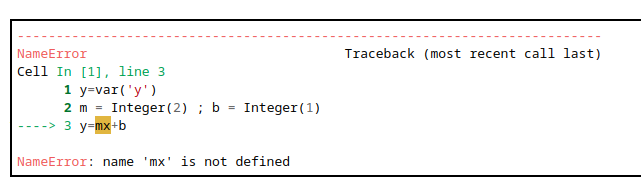
\includegraphics[scale=.5]{sage_cell-error.png}

To be fair, Sage usually puts out error messages that are on the cryptic 
side.  But not this time!  The message says ``NameError'' and it's even 
highlighted the thing that's wrong. 

%\footnote{A takeaway from this is that 
%you can't rely on implicit multiplication.  If you write \verb+7x+ the 
%system is going to think you've created a new (computer) variable whose 
%name is ``7x.''  What you really {\em meant} was \verb+7*x+ and that's 
%what you have to actually type! } 

If you fix the error, something else a little unexpected happens. Nothing!  There's no output\dots

This is just because the last line is an assignment -- it has no return value.  A very common ``idiom'' you'll see when looking at other people's sage code looks like this:

\begin{codeblock}
\begin{verbatim}
y=var('y')
m = 2 ; b = 1
y=mx+b ; y
\end{verbatim}
\end{codeblock}

\noindent The semicolon is just a way to sneak multiple commands onto a single line.  The difference here (as opposed to the code above) is that the last command isn't the assignment to the variable \verb+y+, it's just \verb+y+ by itself - and that does have a return value, namely the contents of the variable \verb+y+.



	\item Calculate $2^0$, $2^0+2^1$, $2^0+2^1+2^2$, 
		and $2^0+2^1+2^2+2^3$. Continue adding the next
		largest power of $2$ until you notice a pattern in the
		result. What is the pattern?
	
\end{enumerate}


\end{worksheet}
\clearpage



\section{Sage on CoCalc}

For more advanced calculations that require multiple
steps, it will be beneficial to signup for CoCalc. CoCalc is a cloud-based service\footnote{``In the cloud'' really just means ``on somebody else's computer.''  There are a ton of servers out there that can be rented on flexible terms, CoCalc just purchases computing power as needed\dots} that gives its users access to many software packages.  Originally it was Sage only, but now, in addition to Sage,  one can run Python notebooks, \LaTeX{} documents, get a full Linux terminal, run a so-called ``computational whiteboard,'' even manage a course on CoCalc.  The CoCalc interface allows for sharing projects and working on thing collaboratively with one's partners -- edits become visible to the other party in real time.

Because of its genesis as a web interface to a free, open-source project, CoCalc makes free accounts available.  One can also purchase ``upgrades'' that give certain perks (most notably, access to less highly-loaded servers for your computations).  The free accounts come equipped with an ``annoyatron'' banner that urges you to get a payed account.  Many Colleges/Universities will be able to provide you with upgrade tokens so you will have the more premium experience.


This lab will lead you through the process of obtaining a CoCalc account and getting started with the Sage notebook interface.

\clearpage
\begin{worksheet}{7}{Sage on CoCalc}{sage.png}
\begin{enumerate}
	\item Go to \url{https://cocalc.com/} in a web browser.
	\item At the top right of the screen, click on the ``Sign Up''
		link.
	\item You'll need to check the box that says ``I agree to the Terms of Service.''  There is also a ``Privacy Policy'' that is included by reference into the Terms of Service.
	\item It also asks you to select the software that you plan to use.  At a minimum select ``SageMath.''  There's also an ``Everything!'' option if you feel adventurous.
	\item Next you'll be asked for your email address, your name, and to choose a password -- please make it a strong one!
	\item You should now see a page that says ``Signed in as
		XXXX XXXX'' at the top of the page.
	\item Click on the ``Projects'' link at the top left of the page.
	\item In the textbox that says, ``Project title -- you can easily change
		this at any time!'' enter a name for your new project, then
		click on the ``Create New Project'' button.
	\item On the next page, click the ``New'' link near the top
		of the page.  This is going to let you create a file inside your project.
	\item Pick a name for your file, select ``Sage worksheet,''
		then click on the ``Start project'' button at the top of the page.
	\item  Unlike in an
		embedded SageMathCell on a webpage, CoCalc will provide
		output for multiple calculations at once, and it will allow you to
		keep previous calculations on the screen so that you can
		change them or refer back to them.
	\item The interface you're looking at is called a Sage notebook. A notebook consists of an alternating sequence of input and output cells. There's a thin line between an input cell and the corresponding output cell, and the output cells have a big green border on the left side. Both sorts of cells can be shown or hidden using the little triangles in the left margin. When you first start up a fresh notebook, there is only the first input cell (with a line numbered 1 in it).  Try adding \verb%1+1% in that cell.  Watch for the pulsing green ``busy'' signal\footnote{While sage is ``thinking'' the interface provides a visual indication.  A lot of the delay is about CoCalc obtaining and setting up a fresh cloud server to run your project on, so after the first computation things should go a lot faster.} and take note of how the interface changes when you execute the cell.  (To execute, you can either hit the ``Run'' button or hold down the shift key while hitting the Enter key on your keyboard.)

	\item If you hover your mouse over the line before an input cell it will turn blue. If you then click it you'll get a new cell. It's usually a good idea to break tough computations up into manageable chunks. That's what cells are for. Just be aware that the cells in a notebook aren't independent -- if you set a variable to some value in one cell, the other cells will know about that.  Create a new cell above your \verb%1+1% cell and ask Sage to multiply a couple of random number with 10 or so digits each.  Take note of how long the
	``busy'' signal lasts this time.

	\item Let's re-emphasize a quirky thing about Sage -- assigning a value to a variable doesn't create any output. So if you want to have the computer verify that it really did what you just told it to do (i.e. print some output) you need to write the variable a second time.  This often has the form of some long computation followed by a semicolon and the name of a variable.  Try pasting the following into a new cell and hitting Shift$+$Enter.

\begin{codeblock}
\begin{verbatim}
A, P, r, n, t = var('A, P, r, n, t')
P=1000
r=.06
n=12
t=5
A = P * (1 + r/n)^(t*n) ; A
\end{verbatim}
\end{codeblock}

\item Another point that bears repeating: The instructions in a cell need to be executed in order to have any effect.  It's not enough to put your cursor in the cell and push ``Enter'' (that just adds a linebreak, making the cell longer).  You have to hold the ``Shift'' key while pressing ``Enter'' if you're trying to tell the computer to ``Do it!''  (You can also select the cell and click the ``Run'' button in the toolbar, but you'll soon find that Shift$+$Enter is a lot quicker.)

\item There are two very useful ways of getting help within sage: tab completion and help messages.  Tab completion is something you may have encountered in other computer applications. If you type the first few letters of a command and then hit the "Tab" key, the machine will either complete the typing for you, or give you a list of possible completions. Try typing "plo" in the next cell and then hitting "Tab".  You should see that Sage has a \verb+plot()+ function, but also it can do 3-dimensional plots -- and there are many other arcane-looking plots commands!

\item Ok, you just discovered that sage has a \verb+plot+ command -- but how do you use it? For that, it's often a good idea to look at the help message for the command. To get help, just type a question mark after the name of the command (then "Shift+Enter").

\noindent I usually just scroll down through the help message until I find some examples\dots

\item Speaking of examples, the tool bar above the cells is full of them!  Create a fresh cell, then find the ``Plots'' drop-down and select ``Function''  Hit Shift$+$Enter and you should see something like:

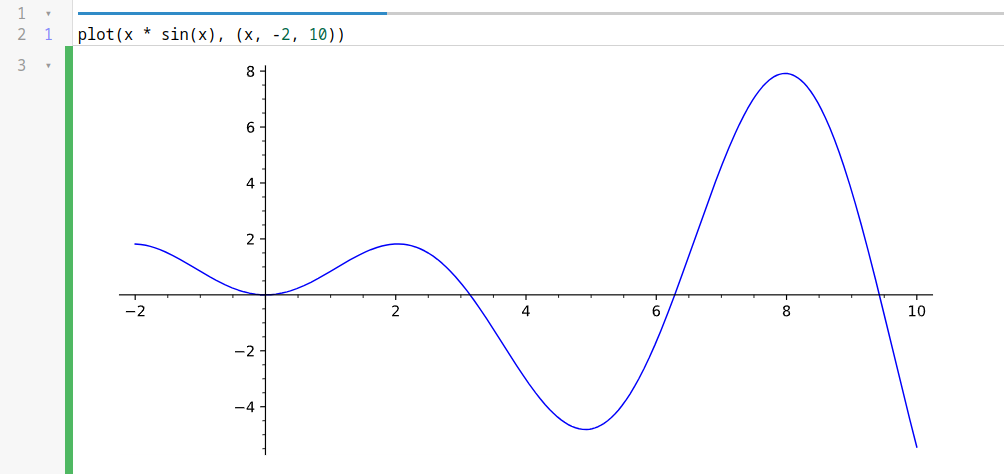
\includegraphics[scale=.4]{first_plot_screenshot.png}

\item Even more help is accessible from the top menu entry that's labelled, uhmmm, ``Help.''  There you can access the sage documentation, submit a support ticket if you think you've found a bug, or even have a chat with ChatGPT.  Try it!

\item When executing a cell produces an error message you can even ask for ``Artificial Intelligence help'' in correcting the problem.  It's possible to hold a back-and-forth conversation with ChatGPT that feels almost like talking to a human!

\item Some of you have probably already studied Calculus.  For others it will be coming up soon! The two main operations in Calculus (which are in a certain sense inverses of one another) are known as integration and differentiation.  Try using tab-completion and the help facility to find out how to do these operations in Sage.  It's pretty likely that you'll do something incorrect and get an error message.  If that happens try the ``Ask ChatGPT'' option.  Turn it into a conversation where you go back and forth with the AI a few times!

\end{enumerate}

\end{worksheet}
\clearpage


Before we start the next lab, some hints about how the interface in CoCalc works are in order.

The interface is called a sage notebook. A notebook consists of an alternating sequence of input and output cells. There's a thin line between an input cell and the corresponding output cell, and the output cells have a big green border on the left side. Both sorts of cells can be shown or hidden using the little triangles in the left margin. 

If you hover your mouse over the line after an output cell it will turn blue. If you then click it you'll get a new cell. It's usually a good idea to break tough computations up into manageable chunks. That's what cells are for. Just be aware that the cells in a notebook aren't independent -- if you set a variable to some value in one cell, the cells below it will know about that.

Let me point out a couple of quirky things:

\begin{enumerate}
	\item The instructions in a cell need to be executed in order to have any effect. It's not enough to put your cursor in the cell and push "Enter" (that just adds a linebreak, making the cell longer). You have to hold the "Shift" key while pressing "Enter" if you're trying to tell the computer to "Do it!"  (You can also select the cell and click the ``Run'' button in the toolbar, but you'll soon find that Shift$+$Enter is a lot quicker.)
	\item The second quirky thing is that assigning a value to a variable doesn't create any output. So if you want to have the computer verify that it really did what you just told it to do (i.e. print some output) you need to write the variable a second time.  This often has the form of some long computation followed by a semicolon and the name of a variable.
\end{enumerate}

begin{codeblock}
\begin{verbatim}
A, P, r, n, t = var('A, P, r, n, t')
P=1000
r=.06
n=12
t=5
A = P * (1 + r/n)^(t*n) ; A
\end{verbatim}
\end{codeblock}

\clearpage
\begin{worksheet}{7}{Sage on CoCalc}{sage.png}
\begin{enumerate}
	\item Go to \url{https://cocalc.com/} in a web browser.
	\item At the top right of the screen, click on the ``Sign Up''
		link.
	\item You'll need to check the box that says ``I agree to the Terms of Service.''  There is also a ``Privacy Policy'' that is included by reference into the Terms of Service.
	\item It also asks you to select the software that you plan to use.  At a minimum select ``SageMath.''  There's also an ``Everything!'' option if you feel adventurous.
	\item Next you'll be asked for your email address, your name, and to choose a password -- please make it a strong one!
	\item You should now see a page that says ``Signed in as
		XXXX XXXX'' at the top of the page.
	\item Click on the ``Projects'' link at the top left of the page.
	\item In the textbox that says, ``Project title -- you can easily change
		this at any time!'' enter a name for your new project, then
		click on the ``Create New Project'' button.
	\item On the next page, click the ``New'' link near the top
		of the page.  This is going to let you create a file inside your project.
	\item Pick a name for your file, select ``Sage worksheet,''
		then click on the ``Start project'' button at the top of the page.
	\item  Unlike in an
		embedded SageMathCell on a webpage, CoCalc will provide
		output for multiple calculations at once, and it will allow you to
		keep previous calculations on the screen so that you can
		change them or refer back to them.
	\item The interface you're looking at is called a Sage notebook. A notebook consists of an alternating sequence of input and output cells. There's a thin line between an input cell and the corresponding output cell, and the output cells have a big green border on the left side. Both sorts of cells can be shown or hidden using the little triangles in the left margin. When you first start up a fresh notebook, there is only the first input cell (with a line numbered 1 in it).  Try adding \verb%1+1% in that cell.  Watch for the pulsing green ``busy'' signal\footnote{While sage is ``thinking'' the interface provides a visual indication.  A lot of the delay is about CoCalc obtaining and setting up a fresh cloud server to run your project on, so after the first computation things should go a lot faster.} and take note of how the interface changes when you execute the cell.  (To execute, you can either hit the ``Run'' button or hold down the shift key while hitting the Enter key on your keyboard.)

	\item If you hover your mouse over the line before an input cell it will turn blue. If you then click it you'll get a new cell. It's usually a good idea to break tough computations up into manageable chunks. That's what cells are for. Just be aware that the cells in a notebook aren't independent -- if you set a variable to some value in one cell, the other cells will know about that.  Create a new cell above your \verb%1+1% cell and ask Sage to multiply a couple of random number with 10 or so digits each.  Take note of how long the
	``busy'' signal lasts this time.

	\item Let's re-emphasize a quirky thing about Sage -- assigning a value to a variable doesn't create any output. So if you want to have the computer verify that it really did what you just told it to do (i.e. print some output) you need to write the variable a second time.  This often has the form of some long computation followed by a semicolon and the name of a variable.  Try pasting the following into a new cell and hitting Shift$+$Enter.

\begin{codeblock}
\begin{verbatim}
A, P, r, n, t = var('A, P, r, n, t')
P=1000
r=.06
n=12
t=5
A = P * (1 + r/n)^(t*n) ; A
\end{verbatim}
\end{codeblock}

\item Another point that bears repeating: The instructions in a cell need to be executed in order to have any effect.  It's not enough to put your cursor in the cell and push ``Enter'' (that just adds a linebreak, making the cell longer).  You have to hold the ``Shift'' key while pressing ``Enter'' if you're trying to tell the computer to ``Do it!''  (You can also select the cell and click the ``Run'' button in the toolbar, but you'll soon find that Shift$+$Enter is a lot quicker.)

\item There are two very useful ways of getting help within sage: tab completion and help messages.  Tab completion is something you may have encountered in other computer applications. If you type the first few letters of a command and then hit the "Tab" key, the machine will either complete the typing for you, or give you a list of possible completions. Try typing "plo" in the next cell and then hitting "Tab".  You should see that Sage has a \verb+plot()+ function, but also it can do 3-dimensional plots -- and there are many other arcane-looking plots commands!

\item Ok, you just discovered that sage has a \verb+plot+ command -- but how do you use it? For that, it's often a good idea to look at the help message for the command. To get help, just type a question mark after the name of the command (then "Shift+Enter").

\noindent I usually just scroll down through the help message until I find some examples\dots

\item Speaking of examples, the tool bar above the cells is full of them!  Create a fresh cell, then find the ``Plots'' drop-down and select ``Function''  Hit Shift$+$Enter and you should see something like:

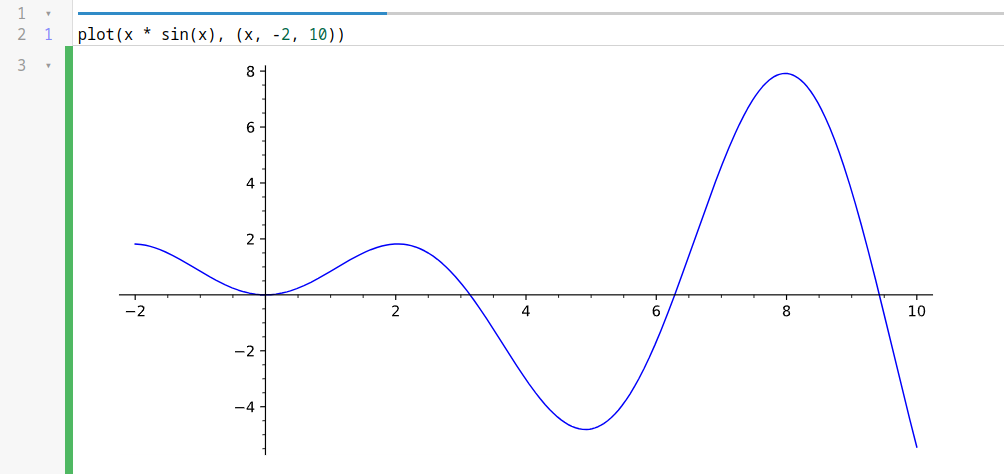
\includegraphics[scale=.4]{first_plot_screenshot.png}

\item Even more help is accessible from the top menu entry that's labelled, uhmmm, ``Help.''  There you can access the sage documentation, submit a support ticket if you think you've found a bug, or even have a chat with ChatGPT.  Try it!

\item When executing a cell produces an error message you can even ask for ``Artificial Intelligence help'' in correcting the problem.  It's possible to hold a back-and-forth conversation with ChatGPT that feels almost like talking to a human!

\item Some of you have probably already studied Calculus.  For others it will be coming up soon! The two main operations in Calculus (which are in a certain sense inverses of one another) are known as integration and differentiation.  Try using tab-completion and the help facility to find out how to do these operations in Sage.  It's pretty likely that you'll do something incorrect and get an error message.  If that happens try the ``Ask ChatGPT'' option.  Turn it into a conversation where you go back and forth with the AI a few times!

\end{enumerate}

\end{worksheet}
\clearpage

\section{Solving equations}

We will investigate functions of the form $f(x)=ax^2+bx+c$. To begin
with, we will consider when $a=1$, $b=0$, and $c=0$, i.e. $f(x)=x^2$.

Start by defining $f(x)=x^2$ in Sage.

\begin{verbatim}
var('x')
f(x)=x^2
\end{verbatim}

To solve the equation $f(x)=1$ (i.e. $x^2=1$) in Sage, we can use the
\textbf{solve} command:

\begin{verbatim}
solve(f(x)==1, x)
\end{verbatim}

This will solve the equation $f(x)=1$, solving for the variable $x$.
Note that when solving, we need to put two equals signs to denote
equality. This is because Sage will interpret a single equals sign
as an assignment (i.e. we would be defining $f(x)$ to be the function
that is always equal to $1$).

The output we obtain is

\begin{verbatim}
[x == -1, x == 1]
\end{verbatim}

These are the two solutions that we expect of $x=-1$ and $x=1$.

\subsection{Practice Exercises}

\begin{enumerate}
	\item Try to solve the equation $f(x)=4$ using Sage.
	\item Solve the equation $f(x)=3$ using Sage.
	\item Solve the equation $f(x)=0$ using Sage.
	\item Do you expect for there to be any solutions for $f(x)=-9$?
		Try it in Sage and see what happens.
	\item For what values of $h$ does $f(x)=h$ have two real solutions?
		Only 1 solution? Two imaginary solutions?
\end{enumerate}

\section{Graphing functions}

Another useful way to visualize functions is by plotting the graph of
functions. Let's begin by plotting the function $f(x)=x^2$:

\begin{verbatim}
var('x')
f(x)=x^2
plot(f(x))
\end{verbatim}

The first two lines define the function $f(x)=x^2$, then the third line will plot
the function. Note that since we did not specify the range for the axes, the
plot will automatically pick a range. If we want to see more of the graph, we
can try adjusting the \textbf{xmin}, \textbf{xmax}, \textbf{ymin}, and \textbf{ymax}
values, which correspond to the minimum and maximum values of the
$x$- and $y$- axes that we desire. For example, changing the plot
command to

\begin{verbatim}
plot(f(x),xmin=-3,xmax=3,ymin=-2,ymax=9)
\end{verbatim}

will gives us an $x$-axis that ranges from $-3$ to $3$ and a $y$-axis that
ranges from $-2$ to $9$.

We can also plot multiple functions on the same plot, in case we
want to compare them together. Let's try overlaying the graph of
the function $g(x)=1$ onto the same set of axes:

\begin{verbatim}
var('x')
f(x)=x^2
g(x)=1
plot([f(x), g(x)],xmin=-3,xmax=3,ymin=-2,ymax=9)
\end{verbatim}

We have defined two functions now, $f(x)=x^2$ and $g(x)=1$. To
plot both, we put them both into a list that is enclosed in square
brackets, with the two functions separated by a comma. This produces
graphs of both $f(x)$ and $g(x)$, in two different colors.

How many times do the graphs of $f(x)$ and $g(x)$ intersect?

\subsection{Practice Exercises}

\begin{enumerate}
	\item Graph the functions $f(x)=x^2$ and $g(x)=4$ together
		on the same set of axes. How many times do the
		graphs of $f(x)$ and $g(x)$ intersect?
	\item Repeat with $f(x)=x^2$ and $g(x)=3$. How many times do the
		graphs of $f(x)$ and $g(x)$ intersect?
	\item Repeat with $f(x)=x^2$ and $g(x)=0$. How many times do the
		graphs of $f(x)$ and $g(x)$ intersect?
	\item Repeat with $f(x)=x^2$ and $g(x)=-9$. How many times do the
		graphs of $f(x)$ and $g(x)$ intersect?
	\item What is the relationship between the number of times
		that the graphs of $f(x)=x^2$ and $g(x)=k$ intersect and the
		number of solutions to $x^2=k$?
\end{enumerate}

\section{Numerical Approximations to Solutions of Equations}

Some equations are difficult to solve exactly even with the
assistant of a computer and computer software, and Sage is no
exception to this. 

Use the \textbf{solve} function to have Sage solve the
equation $x^5-3x^4+x^3+2=0$. 

The output that we get is
\begin{verbatim}
[0 == x^5 - 3*x^4 + x^3 + 2]
\end{verbatim}

which is another way of Sage telling us that it could not find a solution.
However, plotting the function $x^5-3x^4+x^3+2$ tells us another story.
Plot the graph of $x^5-3x^4+x^3+2$ in Sage to see whether it has
any roots. How many are there, and what are the approximate values
from the graph? You may want to play around with the range of the
$x$-axis (using xmin and xmax) to get a clearer picture.

(3 roots, roughly -0.8, 1.2, and 2.5)

We see that there are 3 roots, at roughly $x=-0.8$, $1.2$, and $2.5$.
Although Sage cannot get the exact values for them by solving
the equation $x^5-3x^4+x^3+2=0$, it can get approximate decimal
values for the roots by using the \textbf{find\_root} function. In
short, a computer algebra system such as Sage uses a sophisticated
version of "find where the graph crosses the $x$-axis, and zoom in
repeatedly around that point to get a more precise estimate of the
$x$-coordinate of where the graph crosses the $x$-axis.'' To find
a root $x$ where $-2<x<0$, we would use the command

\begin{verbatim}
find_root(x^5-3*x^4+x^3+2==0, -2, 0)
\end{verbatim}

The output of this is the root

\begin{verbatim}
-0.7931397744702121
\end{verbatim}

If we want to find a different root, we can change the interval on
which we instruct Sage to look for a root. For example, if we want
to find the root near $1.2$, we could try something like

\begin{verbatim}
find_root(x^5-3*x^4+x^3+2==0, 1, 2)
\end{verbatim}

which gives us the value

\begin{verbatim}
1.199258801379252
\end{verbatim}

Try to find the approximate value of the root of $x^5-3x^4+x^3+2$
near $x=2.5$.

(value is 2.563623765649018)

Note that we said that these values are approximate. Let's verify
what we mean by that. Recall that a root of a function $f(x)$ is
a value of $x$ that makes $f(x)$ equal to exactly $0$, i.e.
$f(x)=0$. Use Sage to define the function $f(x)=x^5-3x^4+x^3+2$,
then plug in the values of the approximate roots from above,
e.g. find $f(-0.7931397744702121)$. If $-0.7931397744702121$
is truly a solution to $x^5-3x^4+x^3+2=0$, then
$f(-0.7931397744702121)$ should equal exactly 0.

However, the value that we get from Sage is

\begin{verbatim}
1.35419453428653e-13
\end{verbatim}

The $e$ here is used for \underline{e}ngineering notation,
where 1.35419453428653e-13 means
\begin{equation*}
1.35419453428653\times 10^{-13}
\end{equation*}

In other words, the part before the ``e'' is a decimal number,
but then the part after the ``e'' is the exponent that we should
raise $10$ to then multiply the decimal. Another way to think of
this is that the ``e-13'' means we should start with the
1.35419453428653 then move the decimal to the left 13 times,
making our number smaller. In contrast, if we had seen

\begin{verbatim}1.35419453428653e5\end{verbatim}

that would mean move the decimal to the right 5 places, resulting
in the number $135419.453428653$.

The number $1.35419453428653\times 10^{-13}$ is a really
small number, but it's not exactly equal to 0. This 
demonstrates that the decimal ``solution'' we obtained using
\textbf{find\_root} is only approximate and not an exact solution.

Another thing to be cautious about when using \textbf{find\_root}
is that it will quit as soon as it finds one approximate root. In other
words, even if there is another root in the interval that you specify,
\textbf{find\_root} will only tell you the value of one of them. If we
try

\begin{verbatim}
find_root(x^5-3*x^4+x^3+2==0, 1, 3)
\end{verbatim}

in hopes of finding both roots that are between 1 and 3, it will not
give us both. Try this out and see what you get!

(only the solution 2.563623765649033 is found)

\section{Iterating functions and chaos}

We now consider what happens when applying the function $g(x)=-rx^2+rx$
to a number repeatedly.

We will start when $r=0.5$, so that $g(x)=-0.5x^2+0.5x$. We will start with
the value $x=2$. What is the value of $g(2)$? $g(g(2))$? $g(g(g(2))$?
If we continue to apply $g$ more and more times to the result, what eventually
happens to the output? Use Sage to make your calculations. You may want to
apply \textbf{n()} to your output to get a decimal value to more easily
see the pattern.

Now change $x$ to any number of your choice and repeat the experiment of
applying $g$ repeatedly. What is the eventual outcome?

(all initial values converge to $0$)

Now consider when $r=1.2$, i.e. $g(x)=-1.2x^2+1.2x$.
Start with an initial value of your choice and repeat
the experiment of applying $g$ repeatedly. What is the eventual outcome?

(all initial values converge to $\frac{r-1}{r}=0.1\bar{6}$)

To track the results of iteratively applying the function $g(x)$ to an initial
value of $x=a$, we can create a list of values.

\begin{verbatim}
var('x')
g(x)=-0.5*x^2+0.5*x

a=0.5

points = [a, g(a), g(g(a)), g(g(g(a))), g(g(g(g(a)))), g(g(g(g(g(a)))))]
\end{verbatim}

We can then plot this using the \textbf{list\_plots} function.

\begin{verbatim}
list_plot(points)
\end{verbatim}

If we want to change the value of $a$, we can easily do so, then re-run
the commands that come after it. In addition, if we want to see what
happens when we apply $g(x)$ more times, we can also add those
extra iterates to the list to get a better visualization of what happens
to the output as we apply $g(x)$ more and more times.

Play around with different values of $r$ between $2$ and $4$ and any
choice of the initial value $x$. What patterns do you notice?

Now let's fix a value of $r=3.5$, so we are looking at the function
$g(x)=-3.5x^2+3.5x$. Pick two different values of $x$ that are close to each other 
(within $0.1$ of each other) and plot repeated iterates of $g(x)$ on separate
graphs. What do you notice?
What happens as the two values of $x$ get closer and closer together?

We note that the values seem to be clustered around 4 different values,
and that the iterates seem to cycle through the values systematically. This is called
a \textit{periodic orbit}, and in particular, this is a periodic orbit of length 4 because
the values (approximately) repeat every 4 times that we apply $g$. To find
the periodic points, we can solve for when $x=g(g(g(g(x))))$. Find the points
in this periodic orbit by solving $x=g(g(g(g(x))))$ using Sage.

(Solutions are $x=0, \frac{3}{7}, \frac{5}{7}, \frac{6}{7}$)



\addcontentsline{toc}{chapter}{References}
\phantomsection
\markboth{REFERENCES}{REFERENCES}%
\bibliographystyle{plain}
\bibliography{main}

\addcontentsline{toc}{chapter}{Index} 
\phantomsection
\markboth{INDEX}{INDEX}
\printindex

\end{document}

